\documentclass[onefignum, onetabnum]{siamart190516}
%\usepackage{natbib}
%\usepackage[sort]{cite}
\pdfoutput=1
%\usepackage[colorlinks=true,urlcolor=blue,citecolor=blue,linkcolor=blue]{hyperref}
\usepackage[english]{babel}
\usepackage[utf8]{inputenc}
\usepackage[T1]{fontenc}
\usepackage{amssymb}
\usepackage{tabularx}
\usepackage{quoting}
\usepackage{upquote}
\usepackage{subcaption}
\usepackage{multicol}
\usepackage{cancel}
\usepackage[framemethod=TikZ]{mdframed}
\usetikzlibrary{shapes}
\usetikzlibrary{snakes}
\usepackage{wrapfig}
%\usepackage{caption}
%\usepackage[plain]{algorithmic}
\usepackage[linesnumbered, ruled, vlined, algo2e]{algorithm2e}
\usepackage{algpseudocode}
\usepackage{rotating}
%\usepackage{cite}
\usepackage{booktabs}
%\usepackage{unicode-math}
%\usepackage{algorithm}% http://ctan.org/pkg/algorithm
%\usepackage{algpseudocode}% http://ctan.org/pkg/algpseudocode
\usepackage{xcolor}% http://ctan.org/pkg/xcolor
\makeatletter
\newsavebox{\@brx}
\newcommand{\llangle}[1][]{\savebox{\@brx}{\(\m@th{#1\langle}\)}%
  \mathopen{\copy\@brx\kern-0.5\wd\@brx\usebox{\@brx}}}
\newcommand{\rrangle}[1][]{\savebox{\@brx}{\(\m@th{#1\rangle}\)}%
  \mathclose{\copy\@brx\kern-0.5\wd\@brx\usebox{\@brx}}}
\makeatother
\usepackage{bbm}
\usepackage{jlcode}
\usepackage{graphicx}
\usepackage{amsmath,color}
\usepackage{mathrsfs}
\usepackage{float}
\usepackage[normalem]{ulem}
\usepackage{makecell}
\usepackage{indentfirst}
\usepackage{txfonts}
%\usepackage[epsilon, tsrm, altpo]{backnaur}

\makeatletter
\def\parsept#1#2#3{%
    \def\nospace##1{\zap@space##1 \@empty}%
    \def\rawparsept(##1,##2){%
        \edef#1{\nospace{##1}}%
        \edef#2{\nospace{##2}}%
    }%
    \expandafter\rawparsept#3%
}
\makeatother
\DeclareMathAlphabet{\mymathbb}{U}{BOONDOX-ds}{m}{n}
\newcommand{\listingcaption}[1]%
{%
\refstepcounter{lstlisting}\hfill%
Listing \thelstlisting: #1\hfill%\hfill%
}%
\newcolumntype{b}{X}
\newcolumntype{s}{>{\hsize=.7\hsize}X}
\usepackage{listings}
\lstset{
    language=Julia,
    basicstyle=\ttfamily\scriptsize,
    numberstyle=\scriptsize,
    % numbers=left,
    backgroundcolor=\color{gray!7},
    %backgroundcolor=\color{white},
    %frame=single,
    xleftmargin=2em,
    tabsize=2,
    rulecolor=\color{black!15},
    %title=\lstname,
    escapeinside={(*}{*)},
    breaklines=true,
    %breakatwhitespace=true,
    %framextopmargin=2pt,
    %framexbottommargin=2pt,
    frame=bt,
    extendedchars=true,
    inputencoding=utf8,
    columns=fullflexible,
    %escapeinside={(*@}{@*)},
}

\tolerance=1
\emergencystretch=\maxdimen
\hyphenpenalty=1000
\hbadness=1000

\makeatletter

%%%%%%%%%%%%%%%%%%%%%%%%%%%%%% User specified LaTeX commands.

%Journal reference.  Comma sets off: name, vol, page, year
\def\journal #1, #2, #3, 1#4#5#6{{\sl #1~}{\bf #2}, #3 (1#4#5#6) }
\def\pr{\journal Phys. Rev., }
\def\prb{\journal Phys. Rev. B, }
\def\prl{\journal Phys. Rev. Lett., }
\def\pl{\journal Phys. Lett., }
%\def\np{\journal Nucl. Phys., }


%%%%%%%%%%%%%%%%%%%%%%%%%%%%%%%%%%%%%%%%%%%%%%%%%%%%%%%%%%%%%%%%%%%%%%%%%%%%%%%%%%%%%%%%%%%%%%%%%%%%%%%%%%%%%%%%%%%%%%%%%%%%%%%%%%%%%%%%%%%%%%%%%%%%%%%%%%%%%%%%%%%%%%%%%%%%%%%%%%%%%%%%%%%%%%%%%%%%%%%%%%%%%%%%%%%%%%%%%%%%%%%%%%%%%%%%%%%%%%%%%%%%%%%%%%%%


%\usepackage{CJK}
%\usepackage[colorlinks, citecolor=blue]{hyperref}
\DeclareMathOperator*{\argmax}{arg\,max}

\newcommand{\eqname}[1]{\stepcounter{equation}\tag{\theequation : #1}}
%%%%%% Shortcut related
\newcommand{\<}{\langle}
\renewcommand{\>}{\rangle}
\newcommand{\out}{{\vx^L}}
\newcommand{\inp}{{\vx^0}}
\newcommand{\cquad}{{{ }_{\quad}}}
\newcommand{\pluseq}{\mathrel{+}=}
\newcommand{\minuseq}{\mathrel{-}=}
\newcommand{\vx}{{\mathbf{x}}}
\newcommand{\vg}{{\mathbf{g}}}
\newcommand{\vp}{{\mathbf{p}}}
\newcommand{\vy}{{\mathbf{y}}}
\newcommand{\Var}{{\mathrm{Var}}}
\newcommand{\Mean}{{\mathrm{E}}}
\newcommand{\vvalue}{{\texttt{value}}}
\newcommand{\grad}{{\texttt{grad}}}
\newcommand{\parameter}{{\texttt{parameter}}}
%%%%%% Convention related
\newcommand{\SWAP}{{\rm SWAP}}
\newcommand{\CNOT}{{\rm CNOT}}
\newcommand{\bigO}{{\mathcal{O}}}
\newcommand{\X}{{\rm X}}
\renewcommand{\H}{{\rm H}}
\newcommand{\Rx}{{\rm Rx}}
\renewcommand{\v}[1]{{\bf #1}}
\newcommand{\dataset}{{\mathcal{D}}}
\newcommand{\wfunc}{{\psi}}
\newcommand{\SU}{{\rm SU}}
\newcommand{\UU}{{\rm U}}
\newcommand{\thetav}{{\boldsymbol{\theta}}}
\newcommand{\gammav}{{\boldsymbol{\gamma}}}
\newcommand{\thetai}{{\theta^\alpha_l}}
\newcommand{\Expect}{{\mathbb{E}}}
\newcommand{\Tr}{{\rm Tr}}
\newcommand{\etc}{{\it etc~}}
\newcommand{\etal}{{\it etal~}}
\newcommand{\xset}{\mathbf{X}}
\newcommand{\fl}{\texttt{fl}}
\newcommand{\pdata}{\mathbf{\pi}}
\newcommand{\q}{\mathbf{q}}
\newcommand{\epdata}{\mathbf{\hat{\pi}}}
\newcommand{\gammaset}{\boldsymbol{\Gamma}}
\newcommand{\ei}{{\mathbf{e}_l^\alpha}}
\newcommand{\vtheta}{{\boldsymbol{\theta}}}
\newcommand{\sigmag}{{\nu}}
\newcommand{\sigmai}[2]{{\sigma^{#2}_{#1}}}
\newcommand{\qi}[1]{{q^{\alpha_{#1}}_{#1}}}
\newcommand{\BAS}{Bars-and-Stripes}
\newcommand{\circled}[1]{\raisebox{.5pt}{\textcircled{\raisebox{-.9pt} {#1}}}}
\newcommand{\qexpect}[1]{{\left\langle #1\right\rangle}}
\newcommand{\expect}[2]{{\mathop{\mathbb{E}}\limits_{\substack{#2}}\left[#1\right]}}
\newcommand{\var}[2]{{\mathop{\mathrm{Var}}\limits_{\substack{#2}}\left(#1\right)}}
\newcommand{\pshift}[1]{{p_{\thetav+#1}}}
\newcommand{\upcite}[1]{\textsuperscript{\cite{#1}}}
\newcommand{\Eq}[1]{Eq.~(\ref{#1})}
\newcommand{\Fig}[1]{Fig.~\ref{#1}}
\newcommand{\Lst}[1]{Listing.~\ref{#1}}
\newcommand{\Tbl}[1]{Table~\ref{#1}}
\newcommand{\Sec}[1]{Sec.~\ref{#1}}
\newcommand{\App}[1]{Appendix~\ref{#1}}
\newcommand{\bra}[1]{\mbox{$\left\langle #1 \right|$}}
\newcommand{\ket}[1]{\mbox{$\left| #1 \right\rangle$}}
\newcommand{\braket}[2]{\mbox{$\left\langle #1 | #2 \right\rangle$}}
\newcommand{\tr}[1]{\mathrm{tr}\mbox{$\left[ #1\right]$}}

\newcommand{\ra}[1]{\renewcommand{\arraystretch}{#1}}

%%%%%% Comment related
\newcommand{\red}[1]{[{\bf  \color{red}{ST: #1}}]}
\newcommand{\xred}[1]{[{\bf  \color{red}{\sout{ST: #1}}}]}
\newcommand{\green}[1]{[{\bf  \color{green}{XG: #1}}]}
\newcommand{\xgreen}[1]{[{\bf  \color{green}{\sout{XG: #1}}}]}
\newcommand{\blue}[1]{[{\bf  \color{blue}{JG: #1}}]}
\newcommand{\xblue}[1]{[{\bf  \color{blue}{\sout{JG: #1}}}]}
\newcommand{\material}[1]{\iffalse[{\bf  \color{cyan}{Material: #1}}]\fi}

\newcounter{example}
\newenvironment{example}[1][]{\refstepcounter{example}\par\medskip
   \noindent \textbf{Example~\theexample. #1} \rmfamily}{\medskip}

%\newtheorem{theorem}{\textit{Theorem}}
%\newtheorem{corollary}{\textit Branching Rule}
%\theoremstyle{definition}\newtheorem{definition}{\textit{Definition}}
%\newtheorem{defin}[thm]{Definition}

\makeatother

%\externaldocument{ex_supplement}

\title{Computing properties of independent sets by generic programming tensor networks
\thanks{\funding{...}}
}

\author{XXX\thanks{XXX 
  (\email{email}, \url{website}).}
\and YYY\thanks{yyyyy 
  (\email{yyyy}, \email{email}).}
}

\begin{document}

\maketitle

\begin{abstract}
We introduce a method of using generic programming tensor network to compute various properties of independent sets,
which include the size of the maximum independent sets, the number and enumeration of independent sets and maximal independent sets of a given size.
% which include the size of the maximum independent sets, the number of independent sets and maximal independent sets of a given size, and enumeration of independent sets and maximal independent sets of a given size.
%Although the computational complexity inevitably scales exponentially with treewidth of the graph,
%our method using tensor network contraction with generic programming is highly versatile and is able to compute properties that are otherwise not known to be possible for up to several hundred vertices.
By making use of generic programming, our algorithms are very simple to implement and one can in addition directly utilize recent advances in tensor network contraction techniques such as near-optimal contraction order finding and slicing to achieve high performance.
%One can easily find a good contraction order for the tensor network representation of a graph $G$ with thousands of vertices. 
The algorithmic complexity of this approach is $2^{{\rm tw}(G)}$, where ${\rm tw} (G)$ is the tree width of the problem graph.
Our framework can be easily extended to compute properties of other problems such as the cut size, coloring, and maximal cliques, among others.
To demonstrate the versatility of this tool, we apply it to a few examples including the calculations of the entropy constant for some hardcore lattice gases on 2D square lattices and the overlap gap property on three regular graphs.
\end{abstract}

% REQUIRED
\begin{keywords}
independent set, tensor network, maximum independent set, independence polynomial, generic programming
\end{keywords}

% REQUIRED
% 14N07  	Secant varieties, tensor rank, varieties of sums of powers
\begin{AMS}
  05C31, 14N07
\end{AMS}

\section{Introduction}
In graph theory and combinatorial optimization, there are many interesting and hard computational problems concerning various properties of independent sets.
%An independent set of a graph is a subset of its vertices that no two vertices in this set are adjacent to each other.
For an undirected graph $G = (V,E)$, an independent set $I \subseteq V$ is a set of vertices that for any vertex pair $u,v \in I$, $(u, v) \not\in E$. %there is no edge connecting $u$ and $v$ in $G$. 
One of the independent set properties that many computational complexity theorists are most interested in is to find a maximum independent set (MIS) and the size of the MIS, $\alpha(G) \equiv \max_{I}|I|$. 
\blue{The primary interest of many computational complexity theorists is finding the maximum size of such vertex sets $\alpha(G) \equiv \max_{I}|I|$ and one of the sets of this size.}
Finding $\alpha(G)$ exactly is a hard computational problem, and it is NP-hard even to approximate $\alpha(G)$ within $|V|^{1-\epsilon}$ ~\cite{Hastad1996},
meaning there is unlikely a polynomial time algorithm to find an independent set with size $\alpha(G)/|V|^{1-\epsilon}$ for an arbitrarily small positive $\epsilon$.
Naive exhaustive search for an MIS requires a computational time of $O\left(2^{|V|} \right)$.
More efficient exact algorithms have been developed for finding MISs, such as the branching algorithms~\cite{Tarjan1977, Robson1986} and dynamic programming based algorithms~\cite{Courcelle1990, Fomin2013}.
The branching algorithms can reduce the base of the exponential time scaling to, e.g., $1.1996^{|V|} {|V|}^{O(1)}$~\cite{Xiao2017}, 
while dynamic programming approaches~\cite{Courcelle1990, Fomin2013} works better for graphs with a small treewidth $\text{tw}(G)$, producing algorithms of complexity $O(2^{\text{tw}(G)} \text{tw}(G) |V|)$.
There is immense interest in finding better algorithms to solve the MIS problem, not only because it has 
a wide range of applications in scheduling, logistics, wireless networks and telecommunication, and computer vision, etc.~\cite{Butenko2003, Wu2015}, 
but also because it is a well-known NP-complete problem that can be mapped from many other important combinatorial optimization problems in polynomial time such as the 3-satisfiability problem, the maximum clique problem, and the minimum vertex cover problem~\cite{Moore2011}.

%more concretely, an maximal independent set of a graph $G$ corresponds to a maximum clique in the complement graph of $G$,
%and the complement vertex set of an MIS corresponds to a minimum vertex cover of the graph $G$.
%In this paper, the term ``maximal'' has a different meaning from ``maximum''  which we discussed above; a maximal independent set is an independent set that is not a subset of any other independent set, but its size may not be the maximum.
\blue{We need to distinct ourself in the problem we want to solve.}
In this paper, we do not limit our study to just finding an MIS and its size. 
We introduce a tensor-network based framework to compute the various \textit{properties} pertaining to independent sets.
These properties include, for example, the number and enumeration of independent sets or maximal independent sets of a given size.
We map these independent set problems into generic tensor network contraction with specially designed tensor element algebra.
% There are many other interesting problems pertaining to independent sets, such as the number of independent sets of a given size
% and enumerating independent sets at a give size or what we call computing \textit{properties}.
Some of these problems are of great interest in physics applications such as the hard-core lattice gas model~\cite{Dyre2016, Fernandes2007}
in statistical mechanics and the Rydberg hamiltonian with neutral atoms~\cite{Pichler2018, Ebadi2022} \red{replace with experiment paper when ready};
they can, for example, be used to understand phase transitions, to identify harder graphs in an ensemble of graphs~\cite{Ebadi2022} and to analyze the overlap gap property~\cite{Gamarnik2013, Gamarnik2019}.

Finding the number of independent sets of a given size is equivalent to computing the coefficients of the independence polynomial,
which is a useful graph characteristic related to, for example, the partition functions~\cite{Lee1952,Yang1952} and Euler characteristics of the independence complex~\cite{Bousquet2008, Levit2009}.
The computation of independence polynomials belongs to the complexity class \#P-hard 
and only exponential algorithms~\cite{Ferrin2014} are known to exist for exact computations.
There are also interesting works on efficiently approximating the independence polynomial~\cite{Harvey2018}, but in this work, we focus on exact computations. 
The complexity of our tensor-network based algorithms is similar to that of dynamic programming, which scales exponentially with the treewidth, ${\rm tw}(G)$, of the graph.
% We introduce a tensor-network based framework to compute the various properties pertaining to independent sets.
% We map the independent set problem into generic tensor network contraction with specially designed tensor element algebra.
% Its algorithmic complexity is similar to that of dynamic programming, i.e. scales exponentially as ${\rm tw}(G)$.
%But the tensor network approach is highly versatile so different problems can be generically solved with minimal implementation efforts without loss of efficiency.
We benchmark our algorithms by computing various independent set properties of certain sparse graphs on central processing units (CPUs) and graphics processing units (GPUs); the high performance of our algorithms benefits from recent advances in random tensor-network contraction for the purposes of quantum circuit simulations~\cite{Gray2021, Pan2021, Kalachev2021}.
Algorithms have been developed to optimize the contraction order for tensor networks up to thousands of vertices, which produces a near-optimal space complexity of $2^{\sim{\rm tw}(G)}$ for contracting the tensor network.
For cases where the tensors are too large to fit into a GPU, slicing techniques can be used to further reduce the space consumption.
Lastly, we provide a few examples and demonstrate the versatility of our tool by computing the entropy constant for some hardcore lattice gases on 2D square lattices and analyzing the overlap gap property on three regular graphs.
Our method can also be used to find ``maximal'' independent set properties; 
% Here, the term ``maximal'' has a different meaning from ``maximum''  which we discussed above;
a maximal independent set is an independent set that is not a subset of any other independent set, but its size may not be the maximum. 
We show how to compute properties related to maximal independent sets and properties for other combinatorial optimization problems in \App{app:otherproblems}.

\section{Tensor networks}
Tensor network~\cite{Cirac2020, Orus2014} is also known as einsum, factor graph or sum-product network~\cite{Bishop2006} in different contexts,
it can be viewed as a generalization of matrix multiplication to multiple tensors contraction.
People often use Einstein's notation to represent a tensor network, e.g. the matrix multiplication between two matrices $A$ and $B$ can be represented in Einstein's notation as $C_{ik} = A_{ij}B_{jk}$,
where we use a label in subscripts to represent a degree of freedom.
We enumerate these degree of freedoms and accumulate the product of tensor elements to the output tensor.
In the standard notation of Einstein's summation or tensor network in physics, each index appears precisely twice.
Hence people can represent a tensor network as a simple graph,
where a tensor is a vertex and two tensors sharing the same label are connected.
In the main text, we do not have this restriction. An index can appear arbitrary times.
The graphical representation of our generalized tensor network is hypergraph, in which an edge (label) can be shared by an arbitrary number of vertices (tensors).
These two notations are equivalent in representation power because one can easily translate a generalized tensor network to the standard notation by adding $\delta$ tensors - a high dimensional equivalence of identity matrix.
However, introducing $\delta$ tensors can potentially increase the contraction complexity a lot. We illustrate this point in \App{app:tensorbad}.
\blue{Is it better to introduce the contraction orders here or in example~\ref{eg:tensorcontraction}?}

\begin{example}
$C_{ijk} = A_{jkm} B_{mil} V_{jm}$ is a tensor network that can be evaluated as $C_{ijk} = \sum_{ml}A_{jkm} B_{mil} V_{jm}$.
Its hypergraph representation is shown below, where we use different colors to represent different hyperedges.
%It's equivalent standard notation is $C_{ijk} = A_{ukm} B_{pil} V_{vq} \delta_{mpq} \delta_{juv}\delta_l$. 

\vspace{1em}
\centerline{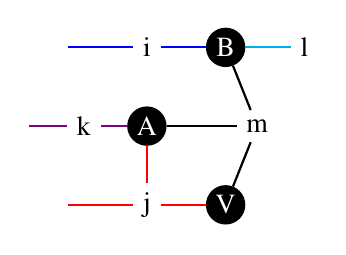
\begin{tikzpicture}[
    dot/.style = {circle, fill, minimum size=#1,
                inner sep=0pt, outer sep=0pt},
    dot/.default = 6pt  % size of the circle diameter 
                    ]  
    \def\dx{0};
    \def\r{0.5cm}
    \def\sr{0.15cm}
    \def\ax{0}
    \def\ay{0}
    \def\bx{1}
    \def\by{1}
    \def\cx{1}
    \def\cy{-1}
    \node[color=white,fill=black,dot=\r] at (\ax+\dx,\ax) (a) {A};
    \node[color=white,fill=black,dot=\r] at (\bx+\dx,\by) (b) {B};
    \node[color=white,fill=black,dot=\r] at (\cx+\dx,\cy) (v) {V};
    \node[color=transparent,draw=transparent,dot=0] at (\ax-1,\by) (o1) {};
    \node[color=transparent,draw=transparent,dot=0] at (\ax-1.5,\ay) (o2) {};
    \node[color=transparent,draw=transparent,dot=0] at (\ax-1,\cy) (o3) {};
    \node at (\ax-0.8,\ay) (k) {k};
    \node at (\bx+0.4,\ay) (m) {m};
    \node at (\ax,\cy) (j) {j};
    \node at (\bx+1,\by) (l) {l};
    \node at (\bx-1,\by) (i) {i};
    \draw[color=blue,thick] (i) -- (b);
    \draw[color=blue,thick] (i) -- (o1);
    \draw[color=cyan,thick] (l) -- (b);
    \draw[color=violet,thick] (k) -- (a);
    \draw[color=violet,thick] (k) -- (o2);
    \draw[color=black,thick] (b) -- (m);
    \draw[color=black,thick] (m) -- (a);
    \draw[color=black,thick] (m) -- (v);
    \draw[color=red,thick] (a) -- (j);
    \draw[color=red,thick] (v) -- (j);
    \draw[color=red,thick] (o3) -- (j);
\end{tikzpicture}}
\end{example}

\section{Generic programming}\label{sec:generic}
In previous works relating tensor networks and combinatoric problems~\cite{Kourtis2019, Biamonte2017},
the elements in the tensor networks are limited to standard number types such as floating point numbers and integers.
Owning to the development of modern compiling technology, we no longer need to limit our imagination to standard number types.
One of the key concepts that push the technology forward is called generic programming:

\begin{definition}[Generic programming ~\cite{Stepanov2014}]
   Generic programming is an approach to programming that focuses on designing algorithms and data structures so that they work in the most general setting without loss of efficiency.
\end{definition}

This definition of generic programming contains two major aspects: a single program works in the most general setting and efficiency.
To understand the first aspect, suppose we want to write a function that raises an element to a power, $f(x, n) := x^n$.
One can easily write a function for standard number types that computes the power of $x$ in $\log(n)$ steps using the multiply and square trick.
Generic programming does not require $x$ to be a standard number type,
instead it treats $x$ as an element with an associative multiplication operation $\odot$ and a multiplicative identity $\mymathbb{1}$.
In such a way, when the program takes a matrix as an input, it computes the matrix power without extra efforts.
The second aspect is about performance. For dynamically typed languages such as Python,
one can easily write very general codes, but the efficiency is not guaranteed; for example, the speed of computing the matrix multiplication between two numpy arrays with python objects as elements is much slower than statically typed languages such as C++ and Julia~\cite{Bezanson2012}.
C++ uses templates for generic programming while Julia takes advantage of just-in-time compilation and multiple dispatch.
When these languages ``see'' a new input type, the compiler can recompile the generic program for the new type.
A myriad of optimizations can be done during the compilation, such as inlining immutable elements with fixed sizes in an array to decrease the cache miss rate when accessing data.
In Julia, these inlined arrays can even be compiled to GPU devices for faster computation~\cite{Besard2018}.

This motivates us to think about what is the most general element type that is allowed in a tensor network contraction program.
We find that as long as the algebra of tensor elements forms a commutative semiring, the tensor network contraction result will be valid and be independent of the contraction order.
A commutative semiring is a semiring with its multiplication operation being commutative, and a semiring is a ring without additive inverse.
To define a commutative semiring with the addition operation $\oplus$ and the multiplication operation $\odot$ on a set $R$, the following relations must hold for any arbitrary three elements $a, b, c \in R$.
\begin{align*}
(a \oplus b) \oplus c = a \oplus (b \oplus c) & \hspace{5em}\text{$\triangleright$ commutative monoid $\oplus$ with identity $\mymathbb{0}$}\\
a \oplus \mymathbb{0} = \mymathbb{0} \oplus a = a &\\
a \oplus b = b \oplus a &\\
&\\
(a \odot b) \odot c = a \odot (b \odot c)  &   \hspace{5em}\text{$\triangleright$ commutative monoid $\odot$ with identity $\mymathbb{1}$}\\
a \odot  \mymathbb{1} =  \mymathbb{1} \odot a = a &\\
a \odot b = b \odot a &\\
&\\
a \odot (b\oplus c) = a\odot b \oplus a\odot c  &  \hspace{5em}\text{$\triangleright$ left and right distributive}\\
(a\oplus b) \odot c = a\odot c \oplus b\odot c &\\
&\\
a \odot \mymathbb{0} = \mymathbb{0} \odot a = \mymathbb{0}
\end{align*}
The requirement of being commutative is for the tensor contraction result to be independent of the contraction order.
In the following sections, we show how to compute the properties of independent sets by designing tensor element types as commutative semirings while keeping the tensor network generic~\cite{Stepanov2014}.
Table~\ref{tbl:generictypes} summarizes the properties that can be solved by various tensor element types. 

\begin{table}[t!]\centering
\begin{minipage}{\columnwidth}
\ra{1.3}
        \begin{tabularx}{\textwidth}{sb}\toprule
            \hline
            \textbf{element type}     & \textbf{property} \\
            {$\mathbbm{R}$}     & {independent sets} \\
            {$\mathbbm{C}$}     & {independence polynomial (approximate)} \\
            {$\text{GF}(p)$} (\Eq{eq:finitefield}) & {independence polynomial} \\
            {T} (\Eq{eq:tropical})    & {MIS size} \\
            {P1} (\Eq{eq:countingtropical})     & {MIS size and the number of MISs} \\
            {P2} (\Eq{eq:max2poly})     & {MISs and independent sets of size $\alpha(G)-1$} \\
            {PN} (\Eq{eq:polynomial})     & {independence polynomial (direct approach)} \\
            {P1+S1}     & {MIS size and one MIS} \\
            {P1+SN} (\Eq{eq:countingtropicalset})    & {MIS size and all MISs} \\
            \bottomrule
        \end{tabularx}
    \caption{Tensor element types and the property we want to calculate when we introduce them.}\label{tbl:generictypes}
\end{minipage}
\end{table}

\section{Independence polynomial}
\subsection{Independence polynomial}\label{sec:indpoly}
The independence polynomial is an important graph polynomial that contains the counting information of independent sets. It is defined as
\begin{equation}\label{eq:idpdef}
I(G, x) = \sum_{k=0}^{\alpha(G)} a_k x^k,
\end{equation}
where $a_k$ is the number of independent sets of size $k$ in $G$. The total number of independent sets is thus equal to $I(G, 1)$.
To compute the independence polynomial of a graph $G = (V, E)$, we reinterpret this problem as a tensor network contraction problem.
We map a vertex $i\in V$ to a label $s_i \in \{0, 1\}$ of dimension $2$ in a tensor network, where we use $0$ ($1$) to denote a vertex absent (exists) in the set.
For each label $s_i$, we defined a parametrized rank-one vertex tensor $W(x_i)$ indexed by it as
\begin{equation}
    W(x_i) = \left(\begin{matrix}
        1 \\
        x_i
    \end{matrix}\right).
\end{equation}
We use subscripts to index tensor elements, e.g. $W(x_i)_0=1$ is the first element associated with $s_i=0$ and $W(x_i)_1=x_i$ is the second element associated with to $s_i=1$.
Similarly, on each edge $(u, v)$, we define a matrix $B$ indexed by $s_u$ and $s_v$ as
\begin{equation}
    \qquad \quad 
       B = \left(\begin{matrix}
        1  & 1\\
        1 & 0
    \end{matrix}\right). \label{eq:edgetensor}
\end{equation}
The corresponding tensor network contraction gives
\begin{equation}\label{eq:idp}
    P(G, \{x_1, x_{2}, \ldots,x_{|V|}\}) = \sum\limits_{s_1, s_2, \ldots, s_{|V|} = 0}^{1} \prod\limits_{i=1}^{|V|} W(x_i)_{s_i} \prod\limits_{(i,j) \in E(G)} B_{s_i s_j},
\end{equation}
where the summation runs over all vertex configurations $\{s_1, s_{2}, \ldots,s_{|V|}\}$ and accumulates the product of tensor elements to the output $P$ (see Example \ref{eg:tensorcontraction} for a concrete example).
The edge tensor element $B_{s_{i}=1, s_{j}=1} = 0$ encodes the independent set constraint, meaning vertex $i$ and $j$ cannot be both in the independent set if they are connected by an edge $(i,j)$.
In the special case of $x_i = x$, the contraction result directly corresponds to the independence polynomial.
The connection can be understood as follows: the product over vertex tensor elements produces a factor $x^k$, where $k=\sum_i s_i$ counts the set size,
and the product over edge tensor elements gives a factor $1$ for a configuration being in an independent set and $0$ otherwise.

%In the implementation of the algorithm, we benefit from recent advances in tensor network contraction,
%where researchers working on quantum circuit simulation evaluate the tensor network by pairwise contracting tensors in a heuristic order~\cite{Gray2021, Pan2021}.
To evaluate \Eq{eq:idp}, summing up the products directly is apparently computational inefficient.
The standard approach to evaluate a tensor network is to contract two tensors a time with a certain order utilizing the associativity and commutativity of tensor elements.
A good contraction order can reduce the time complexity significantly, at the cost of having a space overhead of $O(2^{\text{tw}(G)})$~\cite{Markov2008}.
The pairwise tensor contraction also makes it possible to utilize basic linear algebra subprograms (BLAS) functions to speed up the computation for certain tensor element types.

\begin{example}\label{eg:tensorcontraction}
Mapping a graph (left) to a tensor network (right) that encodes the independence polynomial.
In the generalized tensor network's graphical representation, a vertex is mapped to a hyperedge.
We attach a vertex tensor on each hyperedge and an edge tensor between two hyperedges if vertices of the two hyperedges are connected in the original graph.
    
    \centerline{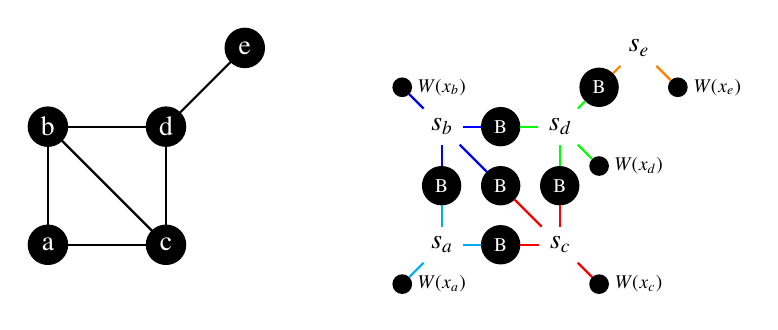
\begin{tikzpicture}[
    dot/.style = {circle, fill, minimum size=#1,
                inner sep=0pt, outer sep=0pt},
    dot/.default = 6pt  % size of the circle diameter 
                    ]  
        \def\dx{0};
        \def\r{0.25cm}
        \filldraw[fill=black] (\dx,0) circle [radius=\r];
        \filldraw[fill=black] (\dx,1.5) circle [radius=\r];
        \filldraw[fill=black] (1.5+\dx,0) circle [radius=\r];
        \filldraw[fill=black] (1.5+\dx,1.5) circle [radius=\r];
        \filldraw[fill=black] (2.5+\dx,2.5) circle [radius=\r];
        \draw [black,thick] (\dx,0) -- (\dx,1.5);
        \draw [black,thick] (\dx,0) -- (1.5+\dx,0);
        \draw [black,thick] (\dx,1.5) -- (1.5+\dx,1.5);
        \draw [black,thick] (1.5+\dx,0) -- (1.5+\dx,1.5);
        \draw [black,thick] (1.5+\dx,0) -- (\dx,1.5);
        \draw [black,thick] (2.5+\dx,2.5) -- (1.5+\dx,1.5);
        \node[color=white] at (\dx,0) {a};
        \node[color=white] at (\dx,1.5) {b};
        \node[color=white] at (1.5+\dx,0) {c};
        \node[color=white] at (1.5+\dx,1.5) {d};
        \node[color=white] at (2.5+\dx,2.5) {e};
        \def\dx{5};
        \def\r{0.25cm}
        \foreach \x/\y/\e in {0.75/0/ac, 0/0.75/ab, 1.5/0.75/cd, 0.75/1.5/bd, 0.75/0.75/bc, 2/2/de}
            \node[color=white,fill=black,dot=2*\r] at (\x+\dx,\y) (\e) {\scriptsize B};
        \foreach \x/\y/\v in {0/0/a, 0/1.5/b, 1.5/0/c, 1.5/1.5/d, 2.5/2.5/e}
            \node[color=black] at (\x+\dx,\y) (\v) {$s_\v$};
        \foreach \x/\y/\v in {-0.5/-0.5/a, -0.5/2.0/b, 2.0/-0.5/c, 2.0/1.0/d, 3.0/2.0/e}
            \node[color=white,fill=black,dot=\r] at (\x+\dx,\y) (\v\v) {};
        \foreach \x/\y/\v in {-0.5/-0.5/a, -0.5/2.0/b, 2.0/-0.5/c, 2.0/1.0/d, 3.0/2.0/e}
            \node[color=black] at (\x+\dx+0.5,\y) {\scriptsize $W(x_\v)$};
        \draw [cyan,thick] (a) -- (aa);
        \draw [cyan,thick] (a) -- (ab);
        \draw [cyan,thick] (a) -- (ac);
        \draw [blue,thick] (b) -- (bb);
        \draw [blue,thick] (b) -- (ab);
        \draw [blue,thick] (b) -- (bc);
        \draw [blue,thick] (b) -- (bd);
        \draw [red,thick] (c) -- (cc);
        \draw [red,thick] (c) -- (ac);
        \draw [red,thick] (c) -- (bc);
        \draw [red,thick] (c) -- (cd);
        \draw [green,thick] (d) -- (dd);
        \draw [green,thick] (d) -- (bd);
        \draw [green,thick] (d) -- (de);
        \draw [green,thick] (d) -- (cd);
        \draw [orange,thick] (e) -- (ee);
        \draw [orange,thick] (e) -- (de);
    \end{tikzpicture}}
    
    The contraction of this tensor network can be done in a pairwise order utilizing the associativity, additive commutativity and multiplicative commutativity of tensor elements:
    \begin{align*}
        &\sum_{s_a,s_b,s_c,s_d,s_e} W(x_a)_{s_a} W(x_b)_{s_b} W(x_c)_{s_c} W(x_d)_{s_d} W(x_e)_{s_e} B_{s_a s_b} B_{s_b s_d} B_{s_c s_d} B_{s_a s_c} B_{s_b s_c} B_{s_d s_e}\\
        =&\sum_{s_b,s_c}\left(\sum_{s_d}\left(\left(\left(\left(\sum_{s_e}B_{s_d s_e}W(x_e)_{s_e}\right) W(x_d)_{s_d}\right) \left(B_{s_bs_d} W(x_b)_{s_b}\right)\right) \left(B_{s_cs_d} W(x_c)_{s_c}\right)\right)\right.\\
        &\phantom{XXX}\left.\left(B_{s_bs_c}\left(\sum_{s_a}B_{s_as_b}\left(B_{s_as_c}W(x_a)_{s_a}\right)\right)\right)\right)\\
        =&1 + x_a + x_b + x_c + x_d + x_e + x_ax_d + x_ax_e + x_cx_e + x_bx_e\\
        =&1+5x+4x^2 \qquad \quad (x_{i} = x)
    \end{align*}
\end{example}

Before contracting the tensor network and evaluating the independence polynomial numerically, let us first elevate the tensor elements $0$s and $1$s in tensors $W(x)$ and $B$ from integers and floating point numbers to the additive identity,
$\mymathbb{0}$, and multiplicative identity, $\mymathbb{1}$, of a commutative semiring as discussed in Sec.~\ref{sec:generic}.
Then we can treat the tensor elements as polynomials and evaluate the polynomial directly.
Let us create a polynomial type, and represent a polynomial $a_0 + a_1 x + \ldots + a_k x^k$ as a coefficient vector $(a_0, a_1, \ldots, a_k) \in \mathbb{R}^k$, so, e.g., $x$ is represented as $(0, 1)$.
We define the algebra between the polynomials $a$ of order $k_a$ and $b$ of order $k_b$ as
\begin{equation}
    \eqname{PN}
    \begin{split}
    a \oplus b &= (a_0 + b_0, a_1 + b_1, \ldots, a_{\max(k_a, k_b)} + b_{\max(k_a, k_b)}),\\
    a \odot b &= (a_0 + b_0, a_1b_0 + a_0b_1, a_{2}b_{0} + a_{1}b_{1} + a_{0}b_{2},  \ldots, a_{k_a} b_{k_b}),\\
    \mymathbb{0} &= (),  \\
    \mymathbb{1} &= (1).\label{eq:polynomial}
    \end{split}
\end{equation}
Here, the multiplication operation can be evaluated efficiently using the convolution theorem~\cite{Schonhage1971}.
We can see these operations are standard addition and multiplication operations of polynomials, and the polynomial type forms a commutative ring. The tensors $W$ and $B$ can thus be written as 
\begin{equation}
    W^{\rm poly} = \left(\begin{matrix}
        \mymathbb{1} \\
        (0,1)
    \end{matrix}\right),   
    \qquad \qquad
        B^{\rm poly} = \left(\begin{matrix}
        \mymathbb{1}  & \mymathbb{1} \\
        \mymathbb{1} & \mymathbb{0}
    \end{matrix}\right).
\end{equation}
By contracting the tensor network with the polynomial type, we have contraction result the exact representation of the independence polynomial.
However, using polynomial numbers suffers from a space overhead proportional to $\alpha(G)$ because each polynomial requires a vector of such size to store the coefficients. 
Here, we propose to find the independence polynomial by fitting $\alpha(G)+1$ random pairs of $x_{i}$ and $y_{i} = I(G,x_{i})$. One can then compute the independence polynomial coefficients $a_{i}$ by solving the linear equation: 
\begin{equation}
\left(\begin{matrix}
1 & x_0 & x_0^2 & \ldots & x_0^{\alpha(G)} \\
1 & x_1 & x_1^2 & \ldots & x_1^{\alpha(G)} \\
\vdots & \vdots & \vdots &\ddots & \vdots \\
1 & x_{\alpha(G)} & x_{\alpha(G)}^2 & \ldots & x_{\alpha(G)}^{\alpha(G)}
\end{matrix}\right)
\left(\begin{matrix}
a_0 \\ a_1 \\ \vdots \\ a_{\alpha(G)}
\end{matrix}\right)
= \left(\begin{matrix}
y_0 \\ y_1 \\ \vdots \\ y_{\alpha(G)}
\end{matrix}\right).\label{eq:lineareq}
\end{equation}
With this approach, we do not incur the linear overhead in space. However, because the independence polynomial coefficients can have a huge order-of-magnitude range, if we use floating point numbers in the computation, the round-off errors can be significant for the counting of large independent set sizes.
In addition, the number could easily overflow if we use fixed-width integer types.
The big integer type is also not a good option because big integers with varying width can be very slow and is incompatible with GPU devices. These problems can be solved by introducing a finite-field algebra $\text{GF}(p)$:
\begin{equation}
\begin{split}
    x ~\oplus~ y &= x+y\pmod p,\\
    x ~\odot~ y &= xy\pmod p,\\
    \mymathbb{0} &= 0,\\
    \mymathbb{1} &= 1.
\end{split}\label{eq:finitefield}
\end{equation}
With a finite-field algebra, we have the following observations:
\begin{enumerate}
    \item One can use Gaussian elimination~\cite{Golub2013} to solve the linear equation \Eq{eq:lineareq} since it is a generic algorithm that works for any elements with field algebra. The multiplicative inverse of a finite-field algebra can be computed with the extended Euclidean algorithm.
    \item Given the remainders of a larger unknown integer $x$ over a set of co-prime integers $\{p_1, p_2, \ldots, p_n\}$,
    $x \pmod {p_1 \times p_2 \times \ldots \times p_n}$ can be computed using the Chinese remainder theorem. With this, one can infer big integers from small integers.
\end{enumerate}
With these observations, we develop Algorithm~\ref{alg:finitefield} to compute the independence polynomial exactly without introducing space overheads.
This is an iterative algorithm that iterates over a sequence of large prime numbers until convergence.
In each iteration, we choose a large prime number $p$, and contract the tensor networks to evaluate the polynomial for each variable $\chi = (x_{0}, x_{1}, \ldots, x_{\alpha(G)})$ on ${\rm GF}(p)$ and denote the outputs as $(y_0, y_1, \ldots, y_{\alpha(G)}) \pmod p$.
Then we solve \Eq{eq:lineareq} using the gaussian elimination on ${\rm GF}(p)$ to find the coefficient modulo $p$, $A_p \equiv (a_0, a_1, \ldots, a_{\alpha(G)})\pmod p$.
As the last step of each iteration, we apply the Chinese remainder theorem to update $A \pmod P $ to $ A \pmod {P\times p}$, where $P$ is a product of all prime numbers chosen in previous iterations.
If this number does not change compared with the previous iteration, it indicates the convergence of result and the program terminates.
All computations are done with integers of fixed width $W$ except the last step of applying the Chinese remainder theorem, where we use arbitrary precision integers to represent the counting.
In \App{app:fft}, we provide another method to solve the linear equation using discrete Fourier transformation.

\LinesNumberedHidden
\begin{algorithm}[!ht]
    \small
    \SetAlgoNoLine
    %\LinesNumbered
    Let $P = 1$, $W$ be the integer width, vector $\chi = (0,1,2, \ldots, \alpha(G))$, matrix $X_{ij} = (\chi_i)^j$, where $i,j = 0, 1, \ldots, \alpha(G)$\;

    \While{true}{
        compute the largest prime $p$ that $\gcd(p, P) = 1$ and $p < 2^W$\;

        \For{$i=0\ldots\alpha(G)$}{
            $y_i \pmod p$ = ${\rm contract\_tensor\_network}(\chi_i\pmod p)$ \tcp*[l]{on $\text{GF}(p)$}
        }

        $A_p = (a_0, a_1, \ldots, a_{\alpha(G)}) \pmod p = {\rm gaussian\_elimination}(X, (y_0, y_1, \ldots, y_{\alpha{G}}) \pmod p) $\;

        $A_{P\times p} = {\rm chinese\_remainder}(A_P, A_p)$\;

        \If{$A_P = A_{P \times p}$}{
            \Return $A_P$ \tcp*[l]{converged}
        }
        $P = P \times p$\;
    }\caption{Computing the independence polynomial exactly without integer overflow}\label{alg:finitefield} 
\end{algorithm}

% \begin{algorithm}[!ht]
%     \small
%     \SetAlgoNoLine
%     %\LinesNumbered
%     Let vector $\chi = (\chi_0,\chi_1,\chi_2, \ldots, \chi_{\alpha(G)})$ be a random sequence, matrix $X_{ij} = (\chi_i)^j$, where $i,j = 0, 1, \ldots, \alpha(G)$\;

%     \For{$i=0\ldots\alpha(G)$}{
%         $y_i$ = ${\rm contract\_tensor\_network}(\chi_i)$
%     }

%     \Return ${\rm gaussian\_elimination}(X, (y_0, y_1, \ldots, y_{\alpha{G}})) $\;
% \end{algorithm}

\section{Maximum independent sets and its counting}
\subsection{Tropical algebra for finding the MIS size and counting MISs}
In the previous section, we focused on computing the independence polynomial for a graph $G$ of given MIS size $\alpha(G)$, but we did not show how to compute this number.
The method we use to compute this quantity is based on the following observations. Let $x=\infty$, the independence polynomial becomes
\begin{equation}
I(G, \infty) = a_{\alpha(G)} \infty^{\alpha(G)},
\end{equation}
where the lower-order terms vanish. We can thus replace the polynomial type $a = (a_0, a_1, \ldots, a_k)$ with new type with two fields: the largest exponent $k$ and its coefficient $a_k$.
From this, we can define a new algebra as
%\begin{equation}
%\begin{split}
%    a(k) \oplus a(j) &= \begin{cases}
%        \left(a_k + a_j, \max(k,j) \right), & k = j \\
%        \left(a_j, \max(k,j) \right), & k < j \\
%        \left(a_k, \max(k,j) \right), & k > j
%    \end{cases}, \\
%    a(k) \odot a(j) &= (a_k a_j, k+j) \\
%    \mymathbb{0} &= (0, -\infty)\\
%    \mymathbb{1} &= (1, 0). \label{eq:countingtropical}
%\end{split}
%\end{equation}
\begin{equation}
    \eqname{P1}
\begin{split}
    a_x\infty^x \oplus a_y\infty^y &= \begin{cases}
        (a_x + a_y)\infty^{\max(x,y)}, & x = y\\
        a_y\infty^{\max(x,y)}, & x < y\\
        a_x\infty^{\max(x,y)}, & x > y
    \end{cases}, \\
    a_x\infty^x \odot a_y\infty^y &= a_x a_y\infty^{x+y}\\
    \mymathbb{0} &= 0\infty^{-\infty}\\
    \mymathbb{1} &= 1\infty^{0}.
\end{split}%& \text{\rlap{(P1)}}
\label{eq:countingtropical}
\end{equation}
To implement this algebra programmatically, we create a data type with two fields $(x, a_x)$ to store the MIS size and its counting,
and define the above operations and constants correspondingly.
When we are only interested in knowing the MIS size, we can drop the counting field.
The algebra of the exponents becomes the max-plus tropical algebra~\cite{Maclagan2015, Moore2011}.:
\begin{equation}\eqname{T}
    \begin{split}
        x \oplus y &= \max(x,y)\\
        x \odot y &= x + y\\
        \mymathbb{0} &= -\infty\\
        \mymathbb{1} &= 0.
    \end{split}\label{eq:tropical}
\end{equation}
This algebra is the same as the one used in Liu et al.~\cite{Liu2021} to calculate and count spin glass ground states.
For independent set calculations here, the vertex tensor and edge tensor becomes:
\begin{equation}
    W^{\rm tropical} = \left(\begin{matrix}
        \mymathbb{1} \\
        \infty
    \end{matrix}\right),   
    \qquad \qquad
        B^{\rm tropical} = \left(\begin{matrix}
        \mymathbb{1}  & \mymathbb{1} \\
        \mymathbb{1} & \mymathbb{0}
    \end{matrix}\right).
\end{equation}

\subsection{Truncated polynomial algebra for counting independent sets of large size}
Instead of counting just the MISs, one may be interested in counting the independent sets of large sizes close to the MIS size.
For example, if one is interested in counting only $a_{\alpha(G)}$ and $a_{\alpha(G)-1}$, we can define a truncated polynomial algebra by keeping only the largest two coefficients in the polynomial in \Eq{eq:polynomial}:
\begin{equation}
    \eqname{P2}
    \begin{split}
    a \oplus b &= (a_{\max(k_a, k_b)-1} + b_{\max(k_a, k_b)-1}, a_{\max(k_a, k_b)} + b_{\max(k_a, k_b)}),\\
    a \odot b &= (a_{k_a-1} b_{k_b}+a_{k_a} b_{k_b-1}, a_{k_a} b_{k_b}),\\
    \mymathbb{0} &= (), \\
    \mymathbb{1} &= (1).\label{eq:max2poly}
    \end{split}
\end{equation}
In the program, we thus need a data structure that contains three fields, the largest order $k$, and the coefficients for the two largest orders $a_k$ and $a_{k-1}$.
This approach can clearly be extended to calculate more independence polynomial coefficients and is more efficient than calculating the entire independence polynomial.
As will be shown below, this algebra can also be extended to enumerate those large-size independent sets.

\section{Enumeration of independent sets}
\subsection{Set algebra for configuration enumeration}
The enumeration problems of independent sets are also interesting and has been studied extensively in the literature~\cite{Bron1973, Eppstein2010, Johnson1988}, including,
for example, the enumeration of all independent sets, the enumeration of all maximal independent sets, or the enumeration of all MISs.
To enumerate all independent sets, we designed an algebra defined on sets of bitstrings.
\begin{equation}
\eqname{SN}
\begin{split}
    s \oplus t &= s \cup t\\
    s \odot t &= \{\sigma \lor^\circ \tau \, | \, \sigma \in s, \tau \in t\}\\
    \mymathbb{0} &= \{\}\\
    \mymathbb{1} &= \{0^{\otimes |V|}\}.
\end{split}\label{eq:set}
\end{equation}
where $s$ and $t$ are each a set of $|V|$-bit strings and $\lor^\circ$ is the bitwise OR operation over two bit strings.
\begin{example}\label{eg:setalgebra}
    For elements being bit strings of length $5$, we have the following set algebra
\begin{equation*}
\begin{split}
    &\{00001\} \oplus \{01110, 01000\} = \{01110, 01000\} \oplus \{00001\} = \{00001,01110, 01000\}\\
    &\{00001\} \oplus \{\} = \{00001\}\\
&\\
    &\{00001\} \odot \{01110, 01000\} = \{01110, 01000\} \odot \{00001\} = \{01111, 01001\}\\
    &\{00001\} \odot \{\} = \{\}\\
    &\{00001\} \odot \{00000\} = \{00001\}
\end{split}
\end{equation*}
\end{example}

To enumerate all independent sets, 
we initialize variable $x_{i}$ in the vertex tensor to $x_i = \{\boldsymbol{e}_{i}\}$, where $\boldsymbol{e}_i$ is a basis bit string of size $|V|$ that has only one non-zero value at location $i$.
The vertex and edge tensors are thus
\begin{equation}
    W^{\rm enum}(\{\boldsymbol{e}_{i}\}) = \left(\begin{matrix}
        \mymathbb{1} \\
        \{\boldsymbol{e}_{i}\}
    \end{matrix}\right),   
    \qquad \qquad
        B^{\rm enum} = \left(\begin{matrix}
        \mymathbb{1}  & \mymathbb{1} \\
        \mymathbb{1} & \mymathbb{0}
    \end{matrix}\right).
\end{equation}

This set algebra can serve as the coefficients in \Eq{eq:countingtropical} to enumerate all MISs, \Eq{eq:polynomial} to enumerate independent sets of different sizes,
or \Eq{eq:max2poly} to enumerate all independent sets of size $\alpha(G)$ and $\alpha(G)-1$.
As long as the coefficients in a truncated polynomial forms a commutative semiring, the polynomial itself is a commutative semiring.
For example, to enumerate only the MISs, with the tropical algebra, we define $s_{k}\infty^k$,
where the coefficient follows the algebra in \Eq{eq:set} and the orders follows the max-plus tropical algebra.
The combined operations become: 
%\begin{equation}
%\begin{split}
%    s(k) \oplus s(j) &= \begin{cases}
%        \left(s_k \cup s_j, \max(k,j) \right), & k = j \\
%        \left(s_j, \max(k,j) \right), & k < j \\
%        \left(s_k, \max(k,j) \right), & k > j
%    \end{cases}, \\
%    s(k) \odot s(j) &= (\{\sigma \lor^\circ \tau \, | \, \sigma \in s_k, \tau \in s_j\}, k+j) \\
%    \mymathbb{0} &= (\{ \}, -\infty)\\
%    \mymathbb{1} &= (\{0^{\otimes |V|}\}, 0). \label{eq:countingtropicalset}
%\end{split}
%\end{equation}
\begin{equation}
\eqname{P1+SN}
\begin{split}
    s_x\infty^x \oplus s_y\infty^y &= \begin{cases}
        (s_x \cup s_y)\infty^{\max(x,y)}, & x = y\\
        s_y\infty^{\max(x,y)}, & x < y\\
        s_x\infty^{\max(x,y)}, & x > y
    \end{cases},\\
    s_x\infty^x \odot s_y\infty^y &= \{\sigma \lor^\circ \tau | \sigma \in s_x, \tau \in s_y\}\infty^{x+y},\\
    \mymathbb{0} &= \{\}\infty^{-\infty},\\
    \mymathbb{1} &= \{0^{\otimes |V|}\}\infty^{0}. \label{eq:countingtropicalset}
\end{split}
\end{equation}
Clearly, the vertex tensor and edge tensor become
\begin{equation}
    W^{\rm MISenum}(\{\boldsymbol{e}_{i}\infty^1\}) = \left(\begin{matrix}
        \mymathbb{1} \\
        \{\boldsymbol{e}_{i}\}\infty^1
    \end{matrix}\right),   
    \qquad \qquad
        B^{\rm MISenum} = \left(\begin{matrix}
        \mymathbb{1}  & \mymathbb{1} \\
        \mymathbb{1} & \mymathbb{0}
    \end{matrix}\right).
\end{equation}
The contraction of the corresponding tensor network yields an enumeration of all MIS configurations.

If one is interested in obtaining only a single MIS configuration, one can just keep a single configuration in the intermediate computations to save the computational effort.
Here is a new algebra defined on the bit strings, replacing the sets of bit strings in \Eq{eq:set}, 
%We leave this as an exercise for readers.
%
%\iffalse
%\begin{equation}
%\begin{split}
%    \sigma_x\infty^x \oplus \sigma_y\infty^y &= \begin{cases}
%        {\rm select}(\sigma_x, \sigma_y)\infty^{\max(x,y)}, & x = y\\
%        \sigma_y\infty^{\max(x,y)}, & x < y\\
%        \sigma_x\infty^{\max(x,y)}, & x > y
%    \end{cases},\\
%    \sigma_x\infty^x \odot \sigma_y\infty^y &= (\sigma_x \lor^\circ \sigma_y)\infty^{x+y},\\
%    \mymathbb{0} &= 1^{\otimes n}\infty^{-\infty},\\
%    \mymathbb{1} &= 0^{\otimes n}\infty^{0},
%\end{split}
%\end{equation}
%\fi
\begin{equation}
\eqname{S1}
\begin{split}
    \sigma \oplus \tau &= {\rm select}(\sigma, \tau), \\
    \sigma \odot \tau &= (\sigma\lor^\circ \tau),\\
    \mymathbb{0} &= 1^{\otimes |V|}, \\
    \mymathbb{1} &= 0^{\otimes |V|},
\end{split}\label{eq:singleconfig}
\end{equation}
where the \texttt{select} function picks one of $\sigma$ and $\tau$ by some criteria to make the algebra commutative and associative, e.g. by picking the one with a smaller integer value.
%In practice, we can just pick randomly from them, in which case the program will output one of the MIS configurations randomly.

% Although the above discussion is in the context of the MIS problem, we can also combine the above algebras with the maximal independence network in \Eq{eq:maximal} to enumerate or sample maximal independent sets,
% as well as other problems in \App{app:otherproblems} for configuration enumeration and sampling.

\subsection{Bounding the MIS enumeration space}
\begin{figure}
    \centering
    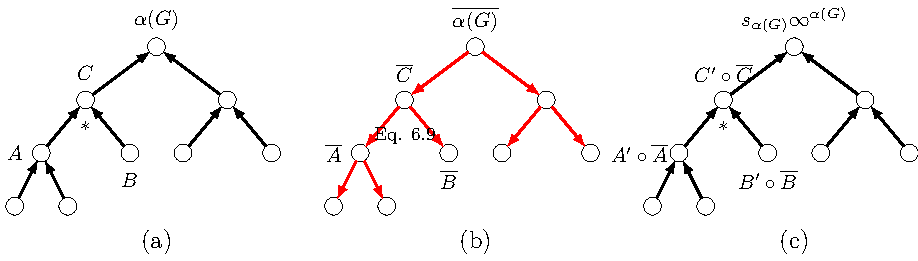
\includegraphics[width=0.9\textwidth, trim={0cm 0cm 0cm 0cm}, clip]{figures/masktree.pdf}
    \caption{Bounded enumeration of maximum independent sets. In the graph, a circle is a tensor, an arrow specifies execution direction of a function and $\circ$ is the Hadamard multiplication. (a) is the forward pass with algebra \Eq{eq:tropical} for computing $\alpha(G)$.
     (b) is the backward pass for computing boolean gradients as masks.
     (c) is the masked forward pass with algebra \Eq{eq:countingtropicalset} for enumerating configurations.}
     \label{fig:bounding}
\end{figure}

When we use the algebra in \Eq{eq:countingtropicalset} to enumerate all MIS configurations, we find that the program stores significantly more intermediate configurations than necessary and thus incur significant overheads in space.
To speed up the computation and reduce space overhead, we bound the searching space using the MIS size $\alpha(G)$.
As shown in \Fig{fig:bounding}, (a) we first compute the value of $\alpha(G)$ with tropical algebra and cache all intermediate tensors.
(b) Then, we compute a boolean mask for each cached tensor, where we use a boolean true to represent a tensor element having a contribution to the MIS (i.e.\ with a non-zero gradient) and boolean false otherwise.
(c) Finally, we perform masked tensor network contraction using the element type with the algebra in \Eq{eq:countingtropicalset} to obtaining all configurations.
Note that these masks in fact correspond to tensor elements with non-zero gradients with respect to the MIS size; we compute these masks by back propagating the gradients.
To derive the back-propagation rule for tropical tensor contraction,
we first reduce the problem to finding the back-propagation rule of a tropical matrix multiplication $C = A B$.
Since $ C_{ik} = \bigoplus_{j} \ A_{ij} \odot B_{jk} = \max_{j} \ A_{ij} \odot B_{jk}$ with tropical algebra, we have the following inequality
\begin{equation}
    A_{ij} \odot B_{jk} \leq C_{ik}.
\end{equation}
Here $\leq$ on tropical numbers are the same as the real-number algebra.
The equality holds for some $j'$, which means $A_{ij'}$ and $B_{j'k}$ have contributions to $C_{ik}$.
Intuitively, one can use this relation to identify elements with nonzero gradients in $A$ and $B$ directly,
however, doing this might make us lost the advantage of using BLAS libraries~\cite{TropicalGEMM}.
Since $A_{ij} \odot B_{jk} = A_{ij} + B_{jk}$, one can move $B_{jk}$ to the right hand side of the inequality: 
\begin{equation}
    A_{ij} \leq C_{ik} \odot B_{jk}^{\circ -1}
\end{equation}
where ${}^{\circ -1}$ is the element-wise multiplicative inverse on tropical algebra (which is the additive inverse on real numbers).
The inequality still holds if we take the minimum over $k$: 
\begin{equation}
    A_{ij} \leq \min_{k}(C_{ik} \odot B_{jk}^{\circ -1}) = \left(\max_{k} \left(C_{ik}^{\circ -1} \odot B_{jk} \right) \right)^{\circ -1} = \left(\bigoplus_{k} \left(C_{ik}^{\circ -1} \odot B_{jk} \right) \right)^{\circ -1} = \left( C^{\circ-1} B^{\mathsf{T}} \right)^{\circ -1}_{ij}.
\end{equation}
On the right hand side, we transform the operation into a tropical matrix multiplication so that we can utilize the fast tropical BLAS routines~\cite{TropicalGEMM}.
Again, the equality holds if and only if the element $A_{ij}$ has a contribution to $C$ (i.e.\ having a non-zero gradient).
Let the gradient mask for $C$ be $\overline C$; the back-propagation rule for gradient masks reads
\begin{equation}\label{eq:adrule}
\overline{A}_{ij} = \delta \left(A_{ij}, \left( \left( C^{\circ-1} \circ \overline C \right) B^{\mathsf{T}} \right)_{ij}^{\circ -1} \right),
\end{equation}
where $\circ$ is the element-wise product, boolean false is treated as the tropical number $\mymathbb{0}$, and boolean true is treated as the tropical number $\mymathbb{1}$.
This rule defined on matrix multiplication can be easily generalized to tensor contraction by replacing the matrix multiplication between $C^{\circ-1} \circ \overline C$ and $B^{\mathsf{T}}$ by a tensor contraction.
With the above method, one can significantly reduce the space needed to store the intermediate configurations by setting the tensor elements masked false to zero during contraction.

\section{Benchmarks and case studies}
\subsection{Performance benchmarks}
We run a single thread benchmark on CPU Intel(R) Xeon(R) CPU E5-2686 v4 @ 2.30GHz,
and its CUDA version on a GPU Tesla V100.
The results are summarized in Figure~\ref{fig:benchmark}.
The graphs that we use in benchmarks are random three regular graphs,
 a typical type of sparse graphs that has a small tree width that asymptotically smaller than $|V|/6$~\cite{Fomin2006}.

\begin{figure} 
    \centering
    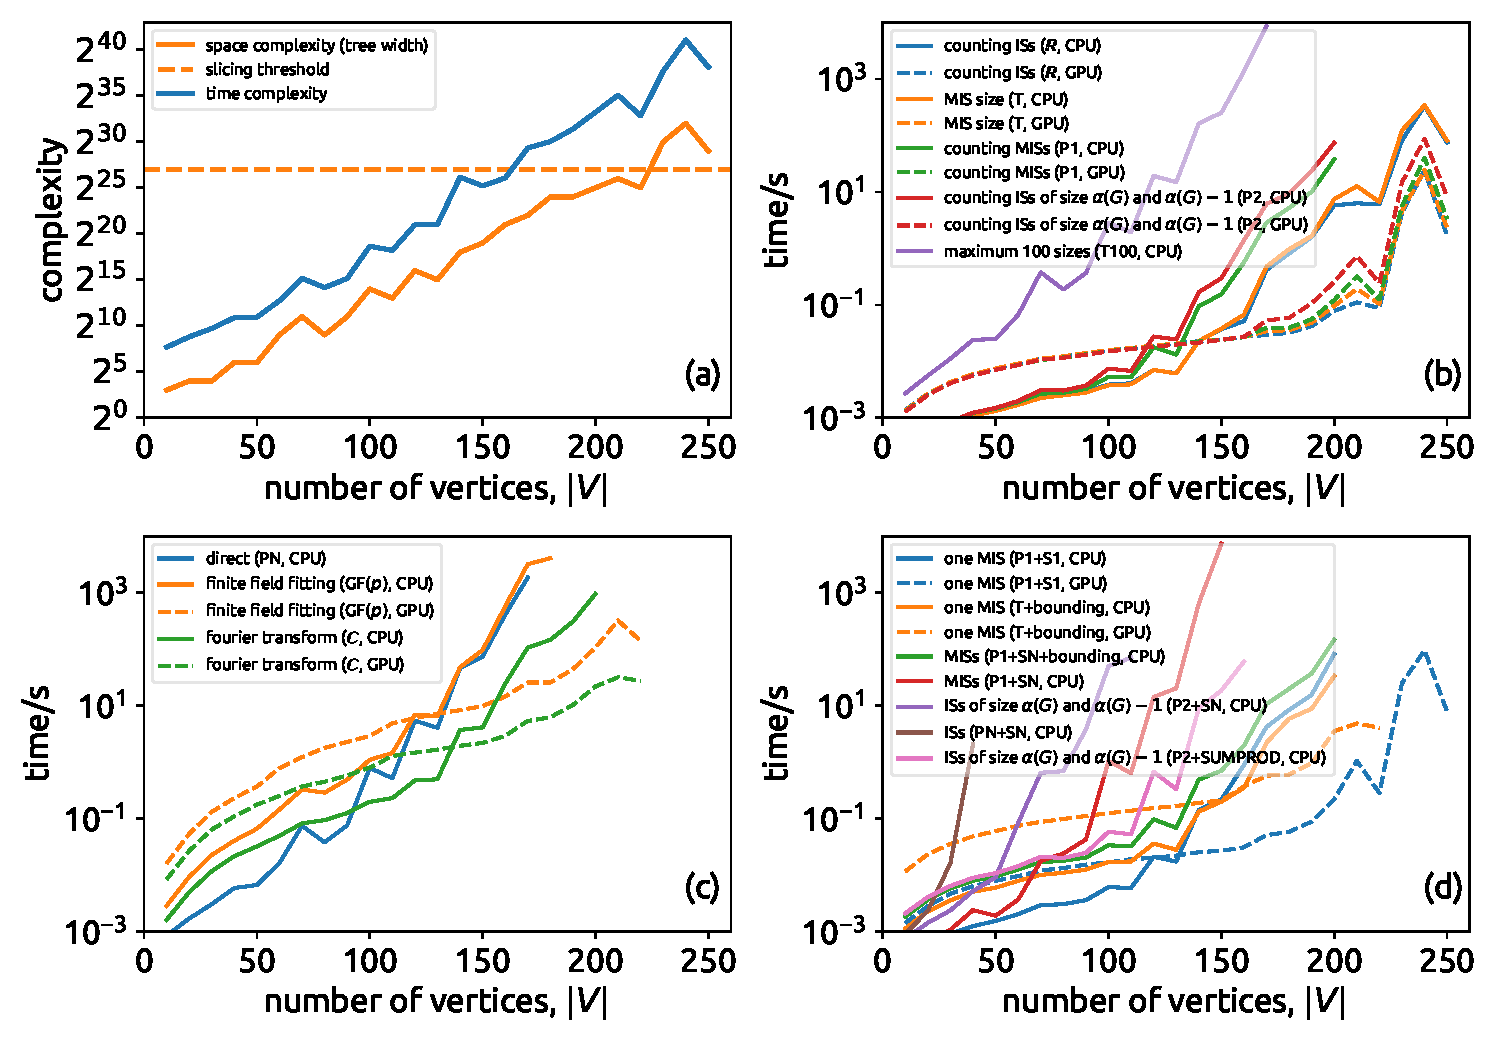
\includegraphics[width=\textwidth, trim={0cm 0cm 0cm 0cm}, clip]{figures/fig1.pdf}
    \caption{Benchmark results for computing different properties of independent sets of a random three regular graph with different tensor element types.
    The time in these plots only includes tensor network contraction, without taking the contraction order finding and just in time compiling time into account.
    Legends are properties, algebra and devices that we used in the computation, one can find the corresponding computed property in \Tbl{tbl:generictypes}.
    (a) time and space complexity versus the number of vertices for the benchmarked graphs.
    (b) The computing time for calculating the MIS size and for counting of the number of independent sets (ISs), the number of MISs, and the number of independent sets having size $\alpha(G)$ and $\alpha(G)-1$ (denoted as ``MISs and (MIS-1)s'').
    (c) The computing time for calculating the independence polynomials with different approaches.
    (d) The computing time for configuration enumeration, including the enumeration of all independent set configurations, a single MIS configuration, all MIS configurations, all independent set configurations having size $\alpha(G)$ and $\alpha(G)-1$,  with or without bounding the enumeration space.
    \red{suggestions for the figure: 1. the legend seems to overlap the lines, especially the large sub-figure. Not sure what's a better way to include the legend there. 2. I see you guys don't typically use markers. We typically use markers to distinguish the different lines, as well as using the color. Especially, for some journals, there is a physical non-color copy, so some requires the figures to be understandable without colors.}
    }
    \label{fig:benchmark}
\end{figure}

Figure (a) shows the time and space complexity (without slicing) of tensor network contraction for variety of graph sizes, where the space complexity is the same as the tree width of the problem graph.
It is obtained with tensor network contraction order optimization algorithm in Ref.~\cite{Kalachev2021}.
In practice, slicing technique is used to fit the computation into a 32GB memory, the target tree width of slicing is $27$.
One can see all the computing times in figure (b), (c) and (d) have a strong correlation with the tree width.
%The computations shown in \Fig{fig:benchmark} include independent set counting, finding maximum independent set size (panel b),
%computing independence polynomial (panel c) and find one independent set and enumerating independent sets (panel d).
Among these benchmarks, computational tasks with data types \texttt{T (CPU)},
\texttt{$\mathbbm{R}$ (CPU)}, \texttt{$\mathbbm{R}$ (GPU)}, \texttt{$\mathbbm{C}$ (CPU)}, \texttt{$\mathbbm{C}$ (GPU)} and \texttt{T+bounding (CPU)} can utilize fast BLAS functions, hence 
are much faster comparing to non-BLAS methods in the same category.
GPU computes much faster than CPU in all cases when the problem scale is large enough so that the actual computing time is comparable or larger than the launching time of CUDA kernels.
Most algebras can be computed on GPU, except those requiring dynamic sized structures, i.e. \texttt{PN} and \texttt{SN}.
In figure (c), one can see the Fourier transformation based method is the fastest in computing the independence polynomial,
however, it maybe suffer from the round off errors. The finite field (GF$(p)$) approach is the only method that does not incur round-off errors and can run on a GPU.
In figure (d), one can see the technique to bound the enumeration space improves the performance for more than one order in enumerating the MISs.
Bounding can also reduce the memory usage significantly, without which the largest computable graph size is only $\sim150$ on a 32GB memory device.

\subsection{Example case studies} In this section, we give a few examples where the different properties of independence sets are used.
In all the examples, the types of graphs we used are shown in Figure~\ref{fig:lattices}, where vertices are all placed on square lattices with lattice dimensions $L \times L$.
The graphs include: the square grid graphs, denoted as SG; the square grid graphs with a filling factor $p$, denoted as SG$(p)$, where $\lfloor pL^{2} \rfloor$ square grids are occupied with vertices;
the King's graphs, denoted as K; the King's graphs with a filling factor $p$, denoted as K$(p)$. 

\begin{figure}[t] 
    \centering
    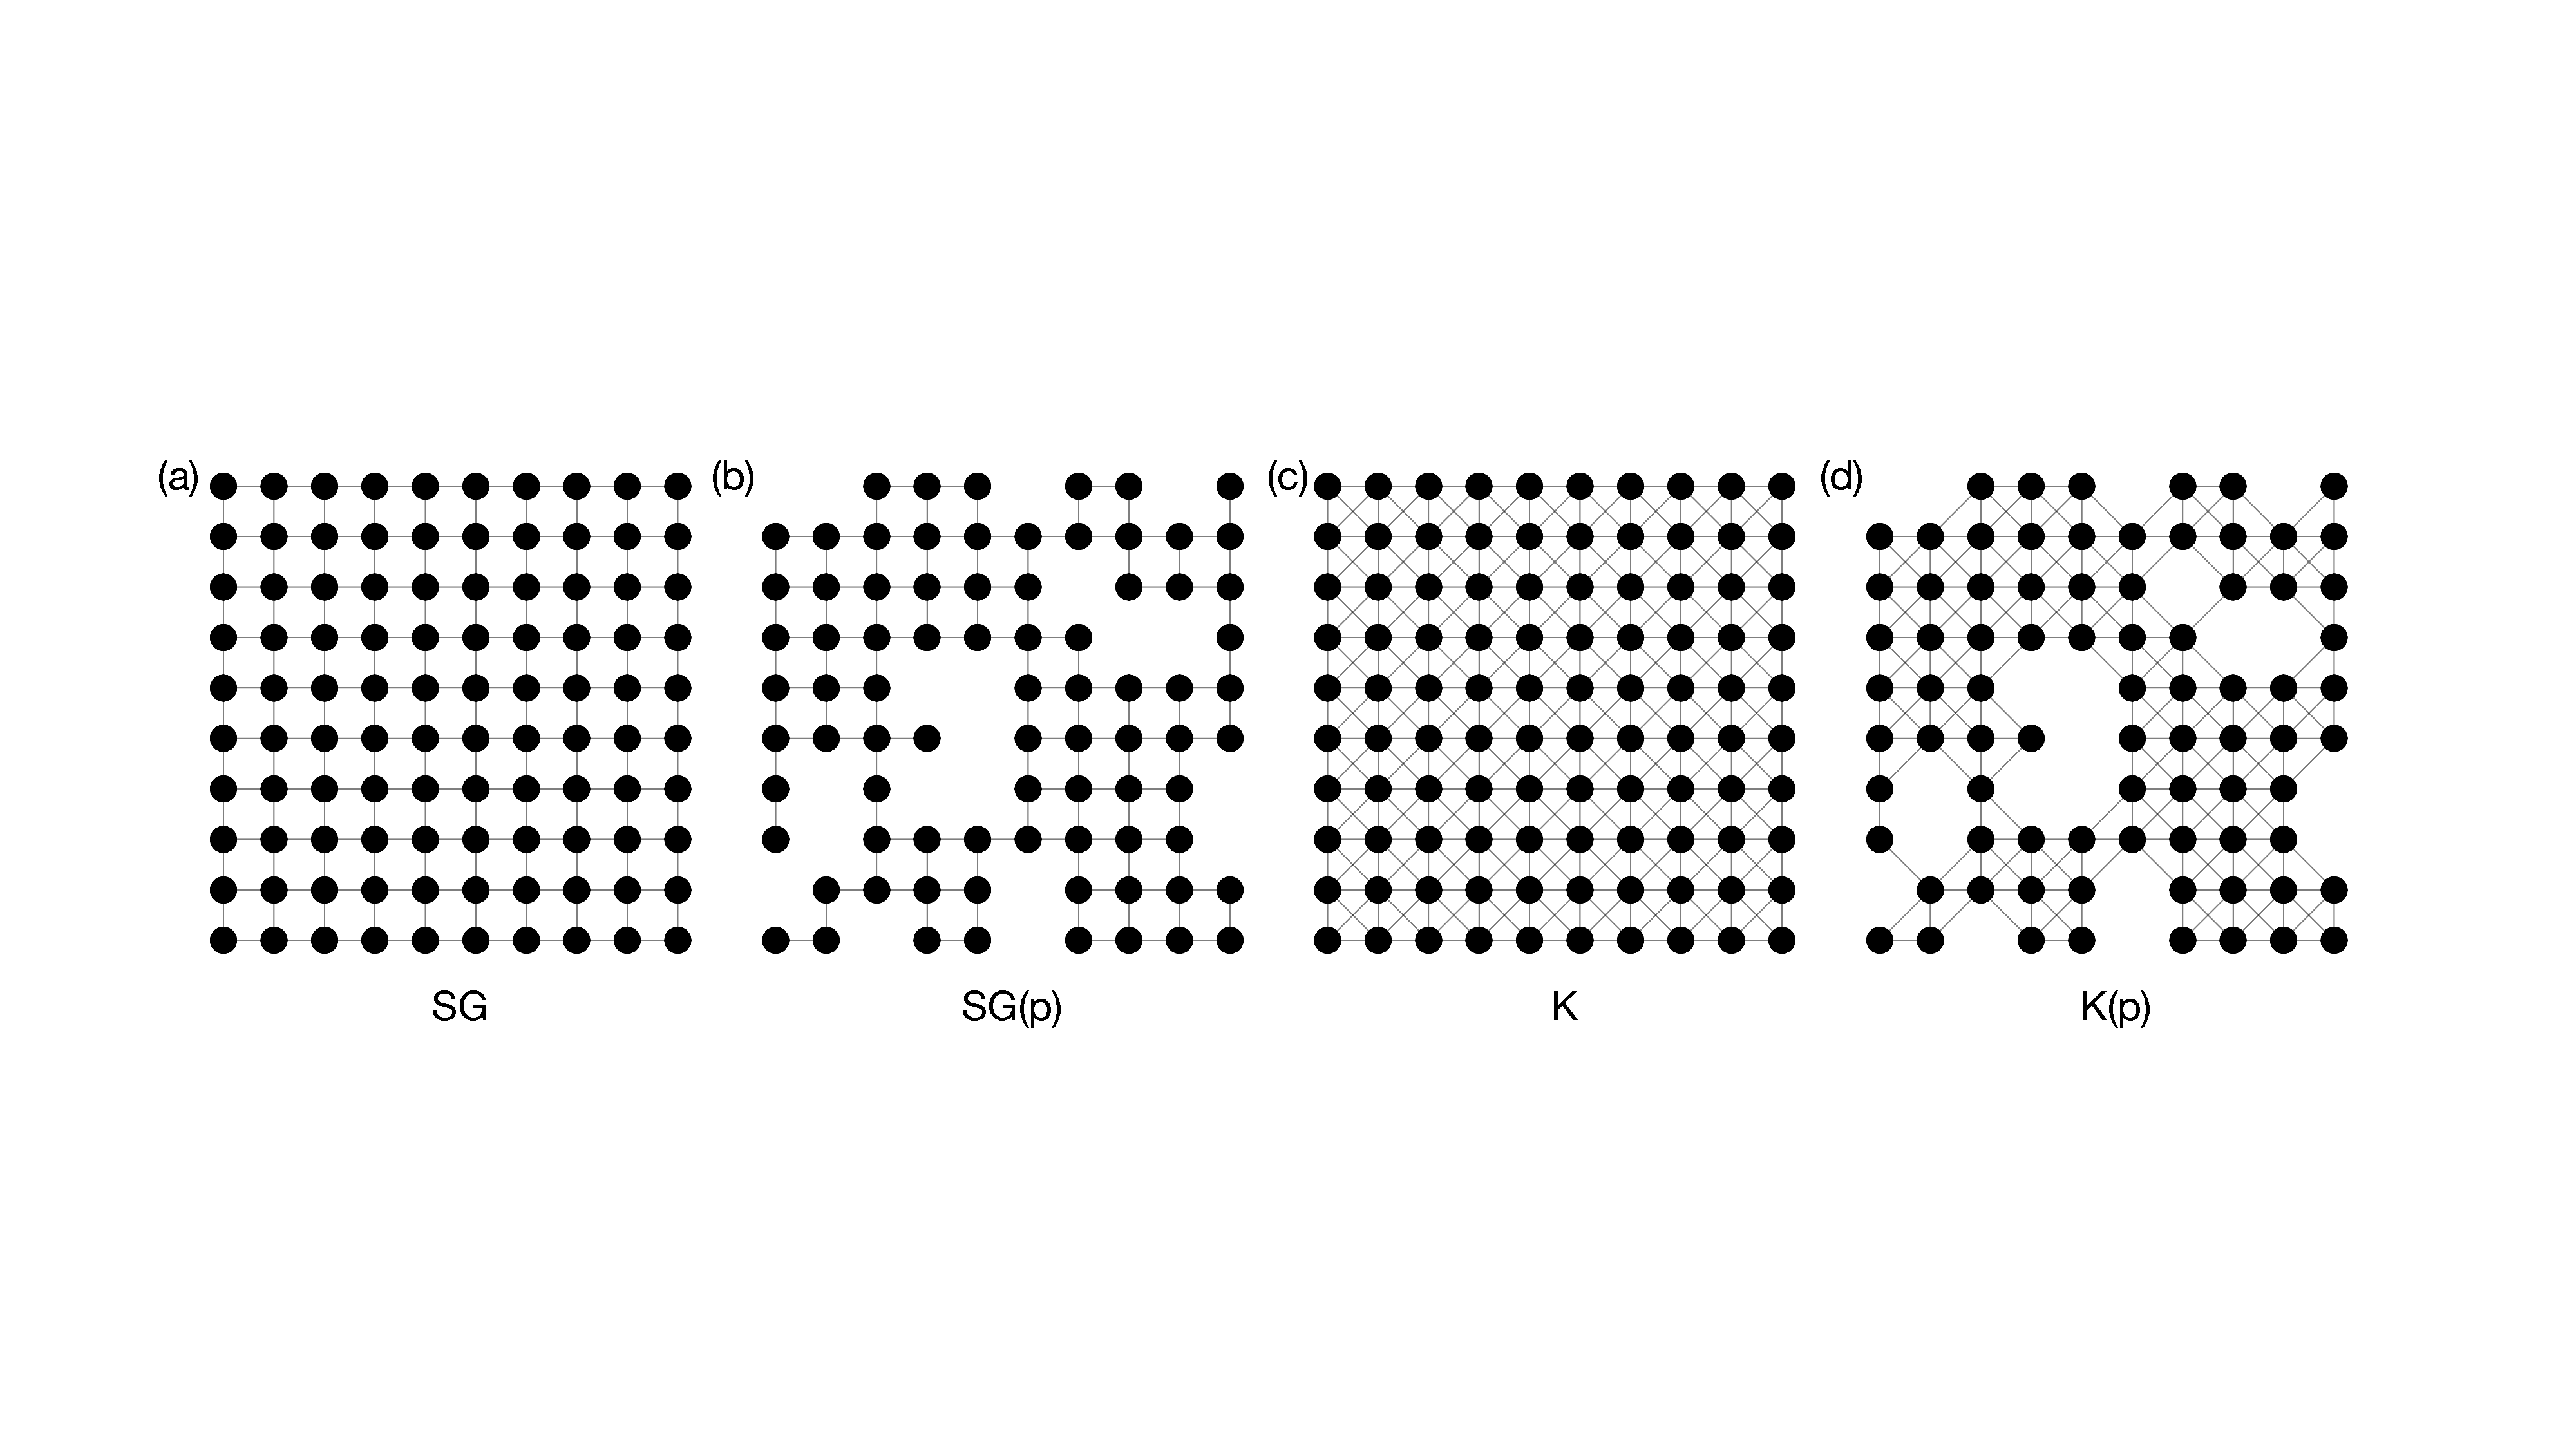
\includegraphics[width=\textwidth, trim={0cm 0cm 0cm 0cm}, clip]{lattices.pdf}
    \caption{The types of graphs used in the benchmark and case studies.
    The lattice dimensions are $L\times L$. (a) Square grid graph denoted as SG. (b) Square grid graph with a filling factor $p=0.8$, denoted as SG(0.8).
    (c) King's graph denoted as K. (d) King's graph with a filling factor $p=0.8$, denoted as K(0.8).}
    \label{fig:lattices}
\end{figure}

\begin{figure}[t] 
    \centering
    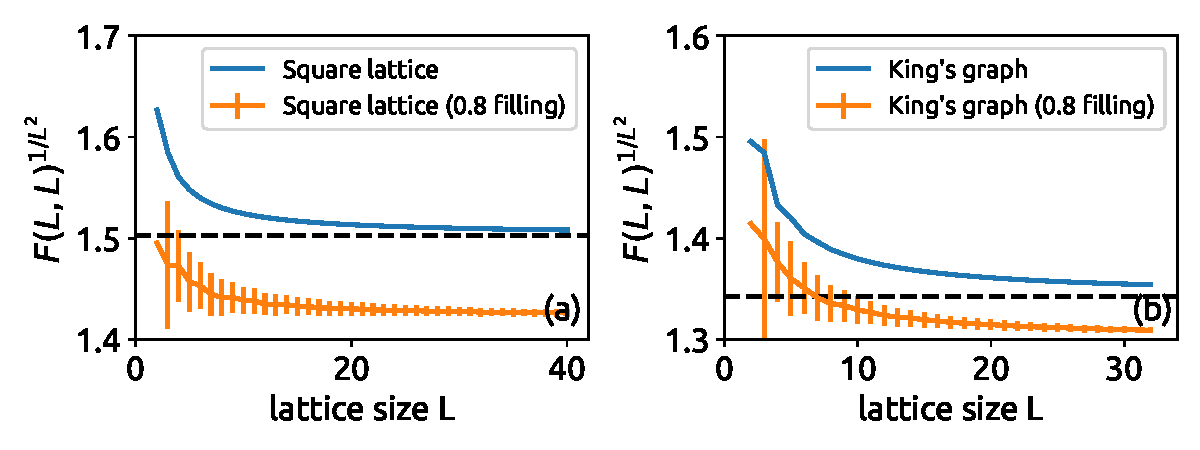
\includegraphics[width=\textwidth, trim={0cm 0cm 0cm 0cm}, clip]{figures/fig5.pdf}
    \caption{Square square entropy constants for lattices defined in \Fig{fig:lattices}, the error bar is scaled by a factor of $1000$.}
    \label{fig:lattices}
\end{figure}

\subsubsection{Number of independent sets and hard-square entropy constant}
The number of independent sets for square grid graphs of size $L \times L$ form a well-known integer sequence (\href{https://oeis.org/A006506}{OEIS A006506}), which is thought as a two-dimensional generalization of the Fibonacci numbers.

\subsubsection{Computing the overlap gap property}

With the ability to enumerate configurations, we can analyse the landscape of the target problem, like the overlap gap property~\cite{Gamarnik2013, Gamarnik2019}.
We compute all MIS and MIS-1 configurations for two random 3 regular graph instances of size 100, and show the Hamming distance statistics in \Fig{fig:hamming}.
The multiple peak structure indicates disconnected clusters in the configuration space.
\begin{figure} 
    \centering
    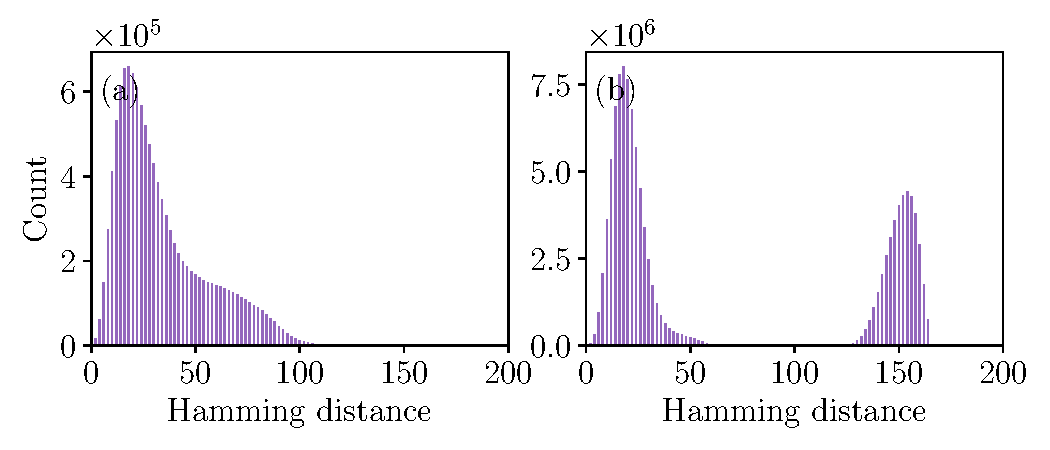
\includegraphics[width=\textwidth, trim={0cm 0cm 0cm 0cm}, clip]{figures/fig3.pdf}
    \caption{The statistics of Hamming distances between two MIS or MIS-1 configurations for two random three regular graph instances of size $100$.}
    \label{fig:hamming}
\end{figure}



\section{Discussion and conclusion}
In this paper, we introduce an abstract algebra formalism to compute properties of independent sets.
The properties include the MIS size, number of independent set of a given size, and enumeration of independent sets of a give size.
For each property, we design a algebra being a commutative semiring, and map the property computation to the contraction of a tensor network with such element type.
%We derived the backward rule for tropical tensor network to bound the search of solution space.
%Although many of these properties are global, we can encode them to different tensor element types as commutative semirings.
We call this method generic programming tensor network, and its power is not limited to the independent set problem.
In \App{app:otherproblems}, we show how to map the maximal independent set problem, matching problem, $k$-colouring problem, max cut problem and set packing problem to tensor networks.
Moreover, since the independence polynomial is closely related to the matching polynomial~\cite{Levit2005}, the clique polynomial~\cite{Hoede1994}, and the vertex cover polynomial~\cite{Akbari2013},
our algorithm to compute the independence polynomial can also be used to compute these graph polynomials.
%Some properties of the independence polynomial, such as the uni-modality, log-concavity, and roots of the polynomial, are well studied in the literature for special classes of graphs~\cite{Levit2005}.
%We hope our algorithms to calculate the independence polynomial can also help further research in these directions.
We show some of the Julia language implementations in Appendix~\ref{sec:technical} and you will find it surprisingly short.
A complete implementation can be found in our Github repository~\cite{GraphTensorNetworks}.
%What we need to do is just defining two operations $\oplus$ and $\odot$ and two special elements $\mymathbb{0}$ and $\mymathbb{1}$.
%The style that we program is called generic programming,

\section*{Acknowledgments}
We would like to thank Pan Zhang for sharing his python code for optimizing contraction orders of a tensor network.
We would like to acknowledge Sepehr Ebadi, Maddie Cain and Leo Zhou for popping up inspiring questions about independent sets,
their questions are driving forces of this project.
Thank Chris Elord for helping us writing the fastest matrix multiplication libary for tropical numbers, TropicalGEMM.jl, he is a man of speed!
Thank other open source software developers: Roger Luo, Time Besard and Katharine Hyatt for solving issues voluntarily.
\blue{funding information}

\bibliographystyle{siamplain}
\bibliography{refs}

\appendix

\section{Technical guide}\label{sec:technical}
This project depends on multiple open source packages in Julia ecosystem.
We list the Julia packages playing important roles in our code base as follows.

\begin{description}
	\item[\href{https://github.com/under-Peter/OMEinsum.jl}{OMEinsum} and \href{https://github.com/Happy-Diode/OMEinsumContractionOrders.jl}{OMEinsumContractionOrders}] are packages providing the support for Einstein's (or tensor network) notation and contraction order optimizations.
    \texttt{OMEinsumContractionOrders} implements state of art algorithms for finding the optimal contraction order for the an tensor network, including the KaHypar+Greedy~\cite{Gray2021, Pan2021} and local transformation based approaches~\cite{Kalachev2021},
	\item[\href{https://github.com/TensorBFS/TropicalNumbers.jl}{TropicalNumbers} and \href{https://github.com/TensorBFS/TropicalGEMM.jl}{TropicalGEMM}] are packages providing tropical number and efficient tropical matrix multiplication,
	\item[\href{https://github.com/JuliaGraphs/Graphs.jl}{Graphs}] is a package providing graph utilities, like random regular graph generator,
	\item[\href{https://github.com/JuliaMath/Polynomials.jl}{Polynomials}] is a package providing polynomial algebra and polynomial fitting,
	\item[\href{https://github.com/scheinerman/Mods.jl}{Mods} and \href{https://github.com/JuliaMath/Primes.jl}{Primes}] are packages providing finite field algebra and prime number generations.
\end{description}

One can install these packages by opening a Julia REPL, type \colorbox{lightgray}{\texttt{]}} to enter the \texttt{pkg>} mode and type, e.g.
\begin{lstlisting}
pkg> add OMEinsum Graphs Mods Primes Polynomials TropicalNumbers OMEinsumContractionOrders
\end{lstlisting}

It may surprise you that the Julia implementation of algorithms introduced in the paper is so short that except the bounding algorithm,
all are contained in this appendix. After installing required packages, one can open a Julia REPL and copy the following code into it.

\lstinputlisting[breaklines]{../democode/demo.jl}

For performance reason, we still recommend checking our GitHub repository for the full featured version:
\href{https://github.com/Happy-Diode/GraphTensorNetworks.jl}{https://github.com/Happy-Diode/GraphTensorNetworks.jl}.
It can be installed in a similar style to other packages. Here is a short introduction to the functionalities in this package.

\lstinputlisting[breaklines]{../democode/tutorial.jl}

\section{The reason to not using the standard tensor network notations}\label{app:tensorbad}
As we have mentioned in the main text,
a standard tensor network notation is equivalent to the generalized tensor network by introducing $\delta$ tensors,
where a $\delta$ tensor of rank $d$ is defined as
\begin{equation}
    \delta_{i_1, i_2,\ldots,i_d} = \begin{cases}
        1, & i_1=i_2=\ldots =i_d,\\
        0, & \text{otherwise}.
    \end{cases}
\end{equation}

Let us consider the following King's graph.

\centerline{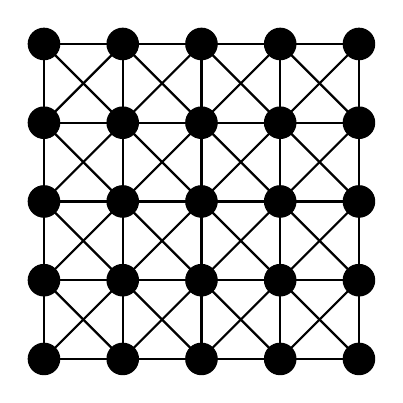
\begin{tikzpicture}
    \def\r{0.2}
    \foreach \x in {1,...,5}
        \foreach \y in {1,...,5}
            \filldraw[fill=black] (\x,\y) circle [radius=\r];
    \foreach \x in {1,...,5}
        \foreach \y in {1,...,4}{
            \draw [black,thick] (\x,\y) -- (\x,\y+1);
            \draw [black,thick] (\y,\x) -- (\y+1,\x);
        }
    \foreach \x in {1,...,4}
        \foreach \y in {1,...,4}{
            \draw [black,thick] (\x,\y) -- (\x+1,\y+1);
            \draw [black,thick] (\y+1,\x) -- (\y,\x+1);
        }
\end{tikzpicture}}

By mapping the independent set problem to a standard tensor network, we have the following graphical representation.

\centerline{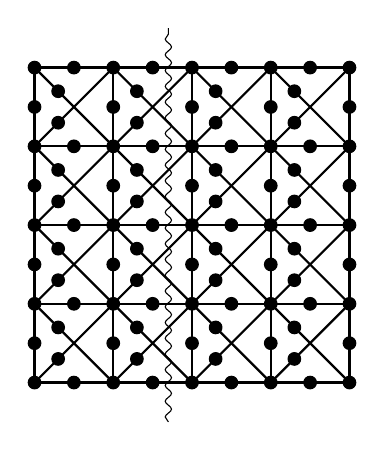
\begin{tikzpicture}
    \def\r{0.08}
    \def\a{0.1}
    \foreach \x in {1,...,5}
        \foreach \y in {1,...,5}
            \filldraw[fill=black] (\x,\y) circle [radius=\r];
    \foreach \x in {1,...,5}
        \foreach \y in {1,...,4}{
            \filldraw[fill=black] (\x,\y+0.5) circle [radius=\r];
            \filldraw[fill=black] (\y+0.5,\x) circle [radius=\r];
            \draw [black,thick] (\x,\y) -- (\x,\y+1);
            \draw [black,thick] (\y,\x) -- (\y+1,\x);
        }
    \foreach \x in {1,...,4}
        \foreach \y in {1,...,4}{
            \filldraw[fill=black] (\x+0.3,\y+0.3) circle [radius=\r];
            \filldraw[fill=black] (\y+0.3,\x+0.7) circle [radius=\r];
            \draw [black,thick] (\x,\y) -- (\x+1,\y+1);
            \draw [black,thick] (\y+1,\x) -- (\y,\x+1);
        }
    \tikzset{decoration={snake,amplitude=.4mm,segment length=2mm,
                    post length=0mm,pre length=0mm}}
    \draw [decorate] (2.7, 0.5) -- (2.7, 5.5);
\end{tikzpicture}}

In this diagram, the circle on each vertex in the original graph is a $\delta$ tensor of rank $8$.
If we contract this tensor network in a naive column-wise order, the maximum intermediate tensor has rank $\sim3L$, requiring a storage of size $\approx 2^{3L}$.
If we relax the restriction that each label appears exactly twice. We have the following hypergraph representation of a generalized tensor network.

\centerline{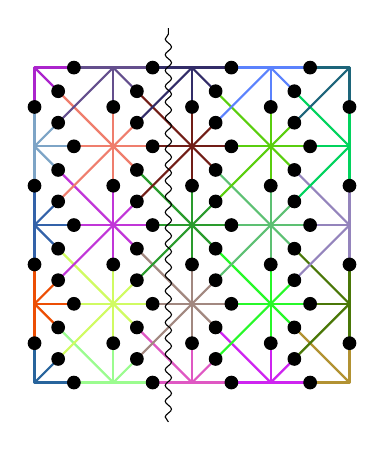
\begin{tikzpicture}
    \def\r{0.08}
    \def\a{0.07}
    \def\L{0.6}
    \def\l{0.1}
    \def\sql{0.24}
    \pgfmathsetseed{2}
    \foreach[evaluate={\cr=0.1+0.5*Mod(\x,2)}] \x in {1,...,5}
        \foreach[evaluate={\cg=0.1+0.3*Mod(\y,2); \cy=0.5-0.5*Mod(\y,2)}] \y in {1,...,5}{
            \edef\R{\pdfuniformdeviate 255}
            \edef\G{\pdfuniformdeviate 255}
            \edef\B{\pdfuniformdeviate 255}
            \xdefinecolor{MyColor}{RGB}{\R,\G,\B}
            \ifnum \x < 5
                \draw [thick, MyColor, opacity=1.0, line cap=round] (\x,\y) -- (\x+0.5,\y);
                \ifnum \y < 5
                \draw [thick, MyColor, opacity=1.0, line cap=round] (\x,\y) -- (\x+0.3,\y+0.3);
                \fi
                \ifnum \y > 1
                \draw [thick, MyColor, opacity=1.0, line cap=round] (\x,\y) -- (\x+0.3,\y-0.3);
                \fi
            \fi
            \ifnum \x > 1
                \draw [thick, MyColor, opacity=1.0, line cap=round] (\x,\y) -- (\x-0.5,\y);
                \ifnum \y < 5
                \draw [thick, MyColor, opacity=1.0, line cap=round] (\x,\y) -- (\x-0.7,\y+0.7);
                \fi
                \ifnum \y > 1
                \draw [thick, MyColor, opacity=1.0, line cap=round] (\x,\y) -- (\x-0.7,\y-0.7);
                \fi
            \fi
            \ifnum \y < 5
                \draw [thick, MyColor, opacity=1.0, line cap=round] (\x,\y) -- (\x,\y+0.5);
            \fi
            \ifnum \y > 1
                \draw [thick, MyColor, opacity=1.0, line cap=round] (\x,\y) -- (\x,\y-0.5);
            \fi
        }
    \foreach \x in {1,...,5}
        \foreach \y in {1,...,5}{
            %\filldraw[fill=black] (\x,\y) circle [radius=0.7*\r];
        }
    \foreach \x in {1,...,5}
        \foreach \y in {1,...,5}{
            \ifnum \y < 5
                \filldraw[fill=black] (\x,\y+0.5) circle [radius=\r];
                \filldraw[fill=black] (\y+0.5,\x) circle [radius=\r];
            \fi
        }
    \foreach \x in {1,...,4}
        \foreach \y in {1,...,4}{
            \filldraw[fill=black] (\x+0.3,\y+0.3) circle [radius=\r];
            \filldraw[fill=black] (\y+0.3,\x+0.7) circle [radius=\r];
        }
    \tikzset{decoration={snake,amplitude=.4mm,segment length=2mm,
                    post length=0mm,pre length=0mm}}
    \draw [decorate] (2.7, 0.5) -- (2.7, 5.5);
\end{tikzpicture}}
Here, we use different colors to distinguish different hyperedges.
A vertex tensor always has rank $1$ and is not shown here since it does not change the contraction complexity.
Again, if we contract this tensor network in the column-wise order, the maximum intermediate tensor rank is $\sim L$, which can be see by counting the number of colors.

\section{Generalizing to other graph problems}\label{app:otherproblems}
%There are some other graph problems that can be encoded to a tensor network.
%To understand its representation power, it is a good starting point to connect it with dynamic programming because
%a tensor network can be viewed as a special type of dynamic programming where its update rule can be characterized by a linear operation.
%Dynamic programming can solve monadic second order logic (MSO) definable problem on a graph with small tree width efficiently~\cite{Courcelle1990,Barr2020}.
%It can solve the maximum independent set problem in $O(2^k)n$, which is similar to the tensor network approach.
%The graph problem can be expressed in the tensor network language is clearly much less than that can be expressed by dynamic programming.
%For example, it is hard to determine whether a collection of vertices forms a path in a graph using the tensor network language, while this problem is MSO definable.
%As a gain, a tensor network has a nicer analytic property, which makes contraction order optimization, generic programming and utilizing BLAS libaries very convenient.
%\iffalse
%The cost is, it is less expressive than MSO because the tensor network described by \Eq{eq:edgetensor} can be expressed in MSO as
%\begin{align}
%    \begin{split}
%    \exists_X\forall_{u}&(\\
%    &\quad\forall_{v} 
%    \neg {\rm adj}(u, v) \lor
%    ({\rm adj}(u, v) \land ( \hspace{5em}\text{$\triangleright$ restrictions on edges}\\
%    &\quad\quad(u \not\in X \land v \not\in X \land B_{00}) \lor\\
%    &\quad\quad(u \not\in X \land v \in X \land B_{01}) \lor\\
%    &\quad\quad(u \in X \land v \not\in X \land B_{10}) \lor\\
%    &\quad\quad(u \in X \land v \in X \land B_{11})\\
%    &\quad)\\
%    &))\land\\
%    &(\hspace{16.5em}\text{$\triangleright$ restrictions on vertices}\\
%    &\quad(u \not\in X \land W_{0}) \lor\\
%    &\quad(u \in X \land W_{1})\\
%    &),
%    \end{split}
%\end{align}
%while not all monadic second order logic can be represented as a tensor network contraction,
%for example, it is hard to construct a tensor network to decide whether a graph is connected or not.
%At the cost of losing expressiveness, we can encode the properties of the graph into the tensor elements.
%\fi
%In the following, we introduce some other problems that can be expressed by a tensor network.
\subsection{Maximal independent sets and maximal cliques}\label{sec:maximal}
Finding maximal independent sets of a graph is equivalent to finding the maximal cliques of its complement graph, so in the following we mainly discuss how to find maximal independent sets.
Let us denote the neighborhood of a vertex $v$ as $N(v)$ and denote $N[v] = N(v)\cup \{v\}$.
A maximal independent set $I_m$ is an independent set where there exists no vertex $v \in V$ such that $I_m \cap N[v]  = \emptyset$.
Similar to the independence polynomial, the maximal independence polynomial counts the number of maximal independent sets of various sizes~\cite{Hu2017},
which can help us understand why the program for solving MIS is trapped in a local minimum.
Concretely, it is defined as
\begin{equation}
I_{\rm max}(G, x) = \sum_{k=0}^{\alpha(G)} b_k x^k,
\end{equation}
where $b_k$ is the number of maximal independent sets of size $k$ in graph $G=(V, E)$.
Comparing with the independence polynomial in \Eq{eq:idpdef}, we have $b_{k} \leq a_{k}$ and $b_{\alpha(G)} = a_{\alpha(G)}$. $I_{\rm max}(G, 1)$ counts the total number of maximal independent sets~\cite{Gaspers2012, Manne2013}, where the fastest algorithm currently has a runtime of $O(1.3642^{|V|})$~\cite{Gaspers2012}.
If we want to find an MIS, $b_{k}$ counts the number of local optimum at size $k < \alpha(G)$, and can, in some cases, provide hints on the difficulty of finding the MIS using local algorithms~\red{cite experiment}.
The uni-modality, log-concavity, and real-rootness properties of the maximal independence polynomial for special classes of graphs have also been studied~\cite{Hu2017}. 

We can modify the tensor network for computing the independence polynomial to include this restriction. Instead of defining the restriction on vertices and edges, it is more natural to define it on $N[v]$:
\begin{equation}\label{eq:maximal}
    T(x_v)_{s_1,s_2,\ldots,s_{|N(v)|},s_v} = \begin{cases}
        s_vx_v & s_1=s_2=\ldots=s_{|N(v)|}=0,\\
        1-s_v& \text{otherwise}.\\
    \end{cases}
\end{equation}
Intuitively, it means if all the neighbourhood vertices are not in $I_{m}$, i.e., $ s_1=s_2=\ldots=s_{|N(v)|}=0$, then $v$ should be in $I_{m}$ and contribute a factor $x_{v}$,
otherwise, if any of the neighbourhood vertices is in $I_{m}$, then $v$ cannot be in $I_{m}$.
As an example, for a vertex of degree 2, the resulting rank-3 tensor is
\begin{equation}
    T(x_v)=\left(\begin{matrix}
    \left(\begin{matrix}
        0 &1 \\
        1 &1
    \end{matrix}\right)\\
    \left(\begin{matrix}
        x_v &0 \\
        0 &0
    \end{matrix}\right)
    \end{matrix}\right).
\end{equation}
 
By contracting this tensor network with generic element type,
we can compute the maximum independent set properties such as maximal independence polynomial, enumerating maximal independent sets.
Let us consider the example in~\Sec{eg:tensorcontraction}: its corresponding tensor network structure for computing the maximal independent polynomial becomes

    \centerline{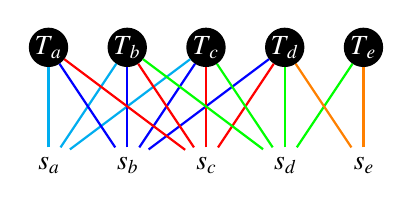
\begin{tikzpicture}[
    dot/.style = {circle, fill, minimum size=#1,
                inner sep=0pt, outer sep=0pt},
    dot/.default = 6pt  % size of the circle diameter 
                    ]  
        \def\dx{0};
        \def\r{0.5cm}
        \def\G{1.0}
        \foreach \x/\y/\v in {0/0/a, 1/0/b, 2/0/c, 3/0/d, 4/0/e}
            \node[color=black] at (\x*\G+\dx,\y) (\v) {$s_\v$};
        \foreach \x/\v/\t in {0/A/$T_a$, 1/B/$T_b$, 2/C/$T_c$, 3/D/$T_d$, 4/E/$T_e$}
            \node[color=white,fill=black,dot=\r] at (\x*\G+\dx,1.5) (\v) {\t};
        \draw [cyan,thick] (a) -- (A);
        \draw [cyan,thick] (a) -- (B);
        \draw [cyan,thick] (a) -- (C);
        \draw [blue,thick] (b) -- (B);
        \draw [blue,thick] (b) -- (A);
        \draw [blue,thick] (b) -- (C);
        \draw [blue,thick] (b) -- (D);
        \draw [red,thick] (c) -- (C);
        \draw [red,thick] (c) -- (A);
        \draw [red,thick] (c) -- (B);
        \draw [red,thick] (c) -- (D);
        \draw [green,thick] (d) -- (D);
        \draw [green,thick] (d) -- (B);
        \draw [green,thick] (d) -- (C);
        \draw [green,thick] (d) -- (E);
        \draw [orange,thick] (e) -- (E);
        \draw [orange,thick] (e) -- (D);
    \end{tikzpicture}}
 
One can see that the average degree of a tensor is increased.
The computational complexity of this new tensor network contraction is often greater than the one for computing the independence polynomial.
However, for most sparse graphs, this tensor network contraction approach is still much faster than enumerating all the maximal cliques on its complement graph using the Bron-Kerbosch algorithm~\cite{Bron1973}, which is the standard algorithm that we are aware of to compute the maximal independence polynomial.
We show the benchmark of computing the maximal independent set properties in \Fig{fig:benchmark-maximal},
including a comparison to the Bron-Kerbosch algorithm from Julia package Graphs~\cite{Graphs}.
%Since the network for computing maximal independent set properties is different from the one for computing the independence polynomial,
the tree width of this tensor network is significantly larger, hence only small graphs can be benchmarked.
The time for the tensor network approach and the Bron-Kerbosch approach to enumerate all maximal independent sets are comparable,
while the tensor network does counting much more efficiently.
Due to the memory limit, this Bron-Kerbosch algorithm stops working at size $70$ and above.

\begin{figure} 
    \centering
    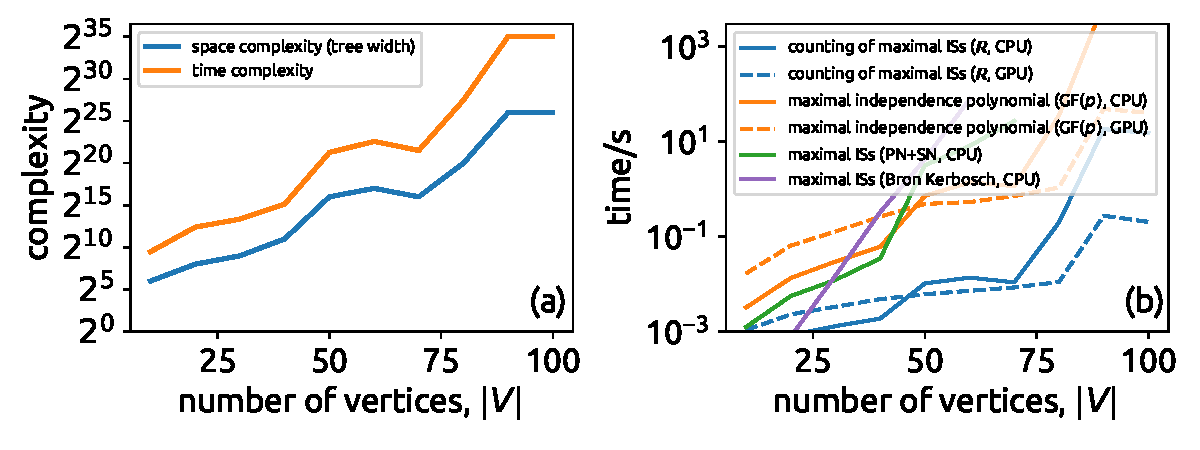
\includegraphics[width=\textwidth, trim={0cm 0cm 0cm 0cm}, clip]{figures/fig2.pdf}
    \caption{Benchmark results for computing different properties of maximal independent sets on a random three regular graph with different tensor element types.
    (a) treewidth versus the number of vertices for the benchmarked graphs. 
    (b) The computing time for calculating the number of independent sets and enumerate all MISs.
    }
    \label{fig:benchmark-maximal}
\end{figure}


\subsection{Matching problem}
A matching polynomial of a graph $G$ is defined as
\begin{equation}
    M(G, x) = \sum\limits_{k=1}^{|V|/2} c_k x^k,
\end{equation}
where $k$ is the number of matches, and coefficients $c_k$ are the corresponding counting.
We map an edge $(u, v) \in E$ to a label $\langle u, v\rangle \in \{0, 1\}$ in a tensor network,
where $1$ means two vertices of an edge are matched, $0$ means otherwise.
Then we define a tensor of rank $d(v) = |N(v)|$ on vertex $v$ such that,
\begin{equation}
    W_{\langle v, n_1\rangle, \langle v, n_2 \rangle, \ldots, \langle v, n_{d(v)}\rangle} = \begin{cases}
        1, & \sum_{i=1}^{d(v)} \langle v, n_i \rangle \leq 1,\\
        0, & \text{otherwise},
    \end{cases}
\end{equation}
and a tensor of rank $1$ on the bond
\begin{equation}
    B_{\langle v, w\rangle} = \begin{cases}
    1, & \langle v, w \rangle = 0 \\
    x, & \langle v, w \rangle = 1,
\end{cases}
\end{equation}
where label $\langle v, w \rangle$ is equivalent to $\langle w,v\rangle$.
Here, a vertex tensor specifies the restriction that a vertex can not be in two matched edges, while an edge tensor contributes the variable in the polynomial.

\subsection{k-Colouring}
Let us use 3-colouring problem defined on vertices as an example.
For a vertex $v$, we define the degree of freedoms $c_v\in\{1,2,3\}$ and a vertex tensor labelled by it as
\begin{equation}
    W(v) = \left(\begin{matrix}
        r_v\\
        g_v\\
        b_v
    \end{matrix}\right).
\end{equation}
For an edge $(u, v)$, we define an edge tensor as a matrix labelled by $(c_u, c_v)$ to specify the constraint
\begin{equation}
    B = \left(\begin{matrix}
        0 & 1 & 1\\
        1 & 0 & 1\\
        1 & 1 & 0
    \end{matrix}\right).
\end{equation}
The number of possible colouring can be obtained by contracting this tensor network by setting vertex tensor elements $r_v, g_v$ and $b_v$ to $1$.
By designing generic types as tensor elements, one can get other properties.
Similarly, one can define the k-colouring problem on edges too by switching the roles of edges and vertices.

\subsection{Max cut problem}
Max cut problem is also known as the boolean spin glass problem.
For a vertex $v\in V$, we define a boolean degree of freedom $s_v\in\{0, 1\}$.
Then the max cut problem can be encoded to tensor networks by mapping an edge $(i,j)\in E$ to an edge matrix labelled by $s_is_j$
\begin{equation}
    B(x_{\langle i, j\rangle}) = \left(\begin{matrix}
        1 & x_{\langle i, j\rangle}\\
        x_{\langle i, j\rangle} & 1
    \end{matrix}\right),
\end{equation}
where variable $x_{\langle i, j\rangle}$ represents a cut on edge $(i, j)$ or a domain wall of an Ising spin glass.
Similar to other problems, we can define a polynomial about edges variables by setting $x_{\langle i, j\rangle} = x$,
where its $k$th coefficient is two times the number of configurations of cut size $k$.

\subsection{Set packing}
Set packing is the hypergraph generalization of the maximum independent set problem, where a set corresponds to a vertex and an element corresponds to a hyperedge.
To solve the set packing problem, we just remove the rank 2 restriction of the edge tensor in \Eq{eq:edgetensor}
\begin{equation}
    B_{v,w,\ldots, z} = \begin{cases}
        1, & v+w+\ldots+z\leq 1,\\
        0, & \text{otherwise}.
    \end{cases}
\end{equation}

\section{The discrete Fourier transform approach to computing the independence polynomial}\label{app:fft}

In section~\ref{sec:indpoly}, we show that the independence polynomial can be obtained by solving the linear equation \Eq{eq:lineareq}.
Since the coefficients of the independence polynomial can range many orders of magnitude, the round-off errors in fitting can be significant if we use random floating point numbers for $x_{i}$.
In the main text, we propose to use a finite field $\text{GF}(p)$ to circumvent integer overflow and round-off errors.
One drawback of using finite field algebra is its matrix multiplication is less computational efficient compared with floating point matrix multiplication.
Here, we give an alternative method based on discrete Fourier transform with controllable round off errors.
Instead of choosing $x_{i}$ as random numbers, we can choose them such that they form a geometric sequence in the complex domain $x_j = r\omega^j$, where $r \in \mathbb{R}$ and $\omega = e^{-2\pi i/( \alpha(G)+1)}$. The linear equation thus becomes
\begin{equation}
\left(\begin{matrix}
1 & r & r^2 & \ldots & r^{\alpha(G)} \\
1 & r\omega & r^2\omega^2 & \ldots & r^{\alpha(G)} \omega^{\alpha(G)} \\
\vdots & \vdots & \vdots &\ddots & \vdots \\
1 & r\omega^{\alpha(G)} & r^2\omega^{2{\alpha(G)}} & \ldots & r^{\alpha(G)}\omega^{{\alpha(G)}^2}
\end{matrix}\right)
\left(\begin{matrix}
a_0 \\ a_1 \\ \vdots \\ a_{\alpha(G)}
\end{matrix}\right)
= \left(\begin{matrix}
y_0 \\ y_1 \\ \vdots \\ y_{\alpha(G)}
\end{matrix}\right).
\end{equation}

Let us rearrange the coefficients $r^j$ to $a_j$, the matrix on the left side becomes the discrete Fourier transform matrix. Thus, we can obtain the coefficients by inverse Fourier transform $\vec a_r = {\rm FFT^{-1}}(\omega) \cdot \vec y$, where $(\vec a_r)_j = a_j r ^j$.
By choosing different $r$, one can obtain better precision in low independent set size region by choosing $r<1$ or high independent set size region by choosing $r>1$.

\section{Integer sequences formed by the number of independent sets}

We computed the number of independent sets on square lattices and King's graphs
with our generic tensor network contraction on GPUs.
The tensor element type is finite field algebra so that we can reach arbitrary precision.
We also computed independence polynomial rigorously for these lattices in our \href{https://github.com/GiggleLiu/NoteOnTropicalMIS/tree/master/data}{Github repo}.


\begin{table}[h]
\caption{The number of independent sets for square grid graphs of size $L\times L$. This forms the integer sequence \href{https://oeis.org/A006506}{OEIS A006506}.
Here we only show two updated entries for $L=38,39$, which to our knowledge, has not been computed before.~\cite{Butera2014}
}
\begin{center}
\scalebox{0.9}{
\begin{tabular}{|c| >{\centering\arraybackslash} p{0.95\linewidth}|}
 \hline $L$  & square grid graphs \\
 \hline $38$ & 616 412 251 028 728 207 385 738 562 656 236 093 713 609 747 387 533 907 560 081 990 229 746 115 948 572 583 817 557 035 128 726 922 565 913 748 716 778 414 190 432 479 964 245 067 083 441 583 742 870 993 696 157 129 887 194 203 643 048 435 362 875 885 498 554 979 326 352 127 528 330 481 118 313 702 375 541 902 300 956 879 563 063 343 972 979\\
 \hline $39$ &  29 855 612 447 544 274 159 031 389 813 027 239 335 497 014 990 491 494 036 487 199 167 155 042 005 286 230 480 609 472 592 158 583 920 411 213 748 368 073 011 775 053 878 033 685 239 323 444 700 725 664 632 236 525 923 258 394 737 964 155 747 730 125 966 370 906 864 022 395 459 136 352 378 231 301 643 917 282 836 792 261 715 266 731 741 625 623 207 330 411 607\\
  \hline
\end{tabular}
}
\end{center}
\label{tbl:squaregrid}
\end{table}
% online digit seperator: https://www.browserling.com/tools/thousands-separator


\begin{table}[h]
\caption{The number of independent sets for King's graphs of size $L\times L$.}
\begin{center}
\begin{tabular}{|c| >{\centering\arraybackslash} p{0.85\linewidth}|}
 \hline $L$  & King's graphs \\
 \hline $ 1$ & 2  \\
 \hline $ 2$ & 5  \\
 \hline $ 3$ & 35  \\
 \hline $ 4$ & 314 \\
 \hline $ 5$ & 6 427 \\
 \hline $ 6$ & 202 841 \\
 \hline $ 7$ & 12 727 570  \\
 \hline $ 8$ & 1 355 115 601 \\
 \hline $ 9$ & 269 718 819 131 \\
 \hline $ 10$ & 94 707 789 944 544 \\
 \hline $ 11$ & 60 711 713 670 028 729  \\
 \hline $ 12$ & 69 645 620 389 200 894 313  \\
 \hline $ 13$ &  144 633 664 064 386 054 815 370 \\
 \hline $ 14$ & 540 156 683 236 043 677 756 331 721  \\
 \hline $ 15$ & 3 641 548 665 525 780 178 990 584 908 643  \\
 \hline $ 16$ & 44 222 017 282 082 621 251 230 960 522 832 336 \\
 \hline $ 17$ & 968 503 939 616 343 947 563 582 929 715 005 880 647 \\
 \hline $ 18$ & 38 227 887 218 717 761 202 510 261 178 854 062 185 464 315 \\
 \hline $ 19$ & 2 720 444 488 584 821 384 410 936 779 813 343 554 469 758 172 682 \\
 \hline $ 20$ & 348 970 226 122 589 397 373 342 369 495 005 120 745 703 462 667 115 175 \\
 \hline $ 21$ & 80 700 603 403 721 730 646 640 814 391 653 008 712 705 595 500 769 624 448 529 \\
 \hline $ 22$ & 33 641 616 174 796 469 294 898 513 022 199 100 689 671 634 779 118 656 571 910 751 320 \\
 \hline $ 23$ & 25 281 578 706 433 684 460 290 055 263 926 749 952 595 755 044 481 112 956 327 672 312 862 611  \\
 \hline $ 24$ & 34 249 181 078 331 384 968 700 380 345 306 575 903 108 280 266 841 066 358 396 857 518 201 026 192 547 \\
 \hline $ 25$ & 83 641 072 313 734 275 009 578 098 702 552 656 178 287 685 025 530 905 558 603 555 359 601 823 180 929 638 318  \\
 \hline $ 26$ & 368 222 048 967 797 645 785 624 418 568 072 838 671 415 214 857 177 141 161 824 615 541 365 640 076 045 923 328 316 979  \\
 \hline $ 27$ & 2 922 282 601 123 898 422 508 409 690 495 824 015 239 663 506 989 438 099 254 205 806 998 557 618 858 143 959 252 475 337 777 029  \\
 \hline $ 28$ & 41 807 680 908 633 213 277 041 952 346 680 116 482 996 387 928 973 684 599 097 559 098 879 721 953 006 036 791 335 134 446 016 561 667 772 \\
  \hline
\end{tabular}
\end{center}
\label{tbl:kingsgrid}
\end{table}

\end{document}
